%%%%%%%%%% Applied Sciences (MDPI) --- SI "Statistics in Data Science: Latest Methods and
%%%%%%%%%% Applications". Reframed draft, started 28 November 2026.
%%
%% Why this file exists. main-mdpi.tex leads with the acquisition floor; this draft leads with the
%% transfer question and keeps the floor as an instrument. The framing is:
%%
%%   context     the VISAPP 2027 result is accepted, reviewed, registered and about to be presented
%%   gap         do corpora of the SAME FORMAT carry it?
%%   hypothesis  they do where the task fixes the figure, and are EQUIVALENT to the bare trace
%%               where the produced shape carries the label
%%   method      the statistics that can tell transfer, equivalence and low power apart, with the
%%               TASK as the unit: thirty slots over six corpora
%%
%% Verdict of the run (addendum I, registered as 4c3eb0e before any number existed): the transfer
%% is real and localised to two slots; the task property does NOT survive being asked within a
%% corpus; equivalence could NOT be claimed for want of precision. Both registered hypotheses of
%% this layer failed, and the paper is written around that.
%%
%% Format. Applied Sciences accepts free-format submission: "We do not have strict formatting
%% requirements, but all manuscripts must contain the required sections." Every required section is
%% present and in the journal's order, with the required back matter. MDPI's own template is
%% deliberately not used while this source is in a repository, because the template licence
%% forbids posting it online; swap it in at revision, when the journal asks for it.
%%
%% Section order note: "Statistical analysis" is its own section between Results and Discussion
%% rather than a subsection of Materials and Methods. That is deliberate for this special issue --
%% the plan and its application are the contribution -- and Materials and Methods points forward
%% to it so a reader looking for the plan in the usual place is not lost.
%%
%% main-mdpi.tex (previous framing) and main.tex (ICML) are untouched. All three share tables/,
%% figures/ and main.bib. The tables are generated by scripts/x3_paper_tables.py in the PDM2
%% research repository and must never be edited here.
%%%%%%%%%%%%%%%%%%%%%%%%%%%%%%%%%%%%%%%%%%%%%%%%%%%%%%%%%%%%%%%%%%%%%%%%%%%%%%%%%%%%%%%%%%%%%%%%

\documentclass[10pt,a4paper]{article}

\usepackage[utf8]{inputenc}
\usepackage[T1]{fontenc}
\usepackage[a4paper,margin=2.5cm]{geometry}
\usepackage{lmodern}
\usepackage{microtype}
\usepackage{graphicx}
\usepackage{subcaption}
\usepackage{booktabs}
\usepackage{amsmath}
\usepackage{amssymb}
\usepackage{mathtools}
\usepackage{amsthm}
\usepackage[numbers,sort&compress]{natbib}
\usepackage{hyperref}
\usepackage[capitalize,noabbrev]{cleveref}

\newtheorem{definition}{Definition}
\setlength{\parskip}{0.4em}
\renewcommand{\arraystretch}{1.1}

% The shared table files are written for the two-column ICML build, where table* is right. Here
% the document is one column and a starred float is page-wide, which LaTeX defers hard. Same
% treatment as main-mdpi.tex: make table* an ordinary float that may sit where the text does.
\makeatletter
\renewenvironment{table*}[1][htbp]{\@float{table}[htbp]}{\end@float}
\makeatother

\renewcommand{\topfraction}{0.9}
\renewcommand{\bottomfraction}{0.8}
\renewcommand{\textfraction}{0.07}
\renewcommand{\floatpagefraction}{0.75}
\setcounter{topnumber}{3}
\setcounter{bottomnumber}{2}
\setcounter{totalnumber}{4}

% Working title. Two alternatives, kept here so the choice is visible rather than silent:
%   Transfer and Equivalence of a Pen-Dynamics Image Encoding Across Six Handwriting Corpora
%   Thirty Tasks, Six Corpora, One Pipeline: Where Does an Image Encoding of Pen Dynamics Transfer?
\title{\bfseries Transfer, Equivalence, or Neither?\\
       A Task-Level Replication of a Pen-Dynamics Image Encoding\\
       Across Six Handwriting Corpora}

% [AUTHOR VERIFICATION REQUIRED]: carried forward from the VISAPP 2027 camera-ready. Confirm
% authorship and order before anything is sent.
\author{%
  Munif Gebara Jr.\,$^{1,*}$,\;
  \'Angel S\'anchez\,$^{2}$,\;
  Yandre Maldonado e Gomes da Costa\,$^{1}$,\\
  Igor Scaliante Wiese\,$^{3}$,\;
  Andr\'e Felipe Ribeiro Cordeiro\,$^{1}$,\;
  Jamily G.\ S.\ Souza\,$^{1}$\\[0.7em]
  \small $^{1}$\,Departamento de Inform\'atica, Universidade Estadual de Maring\'a,
    Maring\'a, PR, Brazil\\
  \small $^{2}$\,Departamento de Inform\'atica y Estad\'istica, Universidad Rey Juan Carlos,
    M\'ostoles, Madrid, Spain\\
  \small $^{3}$\,Departamento de Computa\c{c}\~ao, Universidade Tecnol\'ogica Federal do Paran\'a,
    Campo Mour\~ao, PR, Brazil\\[0.3em]
  \small $^{*}$\,Correspondence: munif@munif.com.br
}
\date{}

\begin{document}
\maketitle

\begin{abstract}
\noindent
A recurring recipe turns a sampled pen trajectory into an image: the path is drawn as ink and a
per-sample signal---speed, pressure, tilt---is painted along it as colour. A published
single-corpus result reported a gain for this encoding in Parkinsonian handwriting. We test whether
it transfers to corpora of the same data format, and where. Twenty-seven candidate corpora were
screened against one criterion---per-sample coordinates with a clock, obtainable by
download---and the seven that qualify were run through one frozen pipeline, with every decision
registered before any metric. Taking the task rather than the corpus as the unit of analysis gives
thirty task slots over six corpora. Two are superior to the bare trace against a margin of $0.03$
declared in advance, both of them prescribed spirals, at $+0.152$ and $+0.119$; neither survives
Holm correction over the thirty, and the only contrast that does is $+0.020$. Pooled over the
thirty slots the encoding is worth $+0.000$ ($I^2 = 53\,\%$). The registered task property---whether
the task fixes the figure---does not account for the margins within a corpus ($-0.009$, exact
$p = 0.391$ of $8{,}008$ enumerated assignments), and task-to-task variation inside a corpus
($\hat\tau = 0.0098$) exceeds corpus-to-corpus variation ($\hat\tau = 0.0067$). Equivalence could
not be claimed: twenty-six of thirty slots cannot resolve $0.03$, and doing so on a clinical task
would take a median of $480$ participants.
\end{abstract}

\noindent\textbf{Keywords:} handwriting; time series to image; transfer; replication; equivalence
testing; two one-sided tests; preregistration; nested cross-validation; heterogeneity; statistical
power; benchmark validity; Parkinson's disease

\vspace{1em}

%%%%%%%%%%%%%%%%%%%%%%%%%%%%%%%%%%%%%%%%%%%%%%%%%%%%%%%%%%%%%%%%%%%%%%%%%%%%%%%%%%%%%%%%%%%%%%%%
%% Introduction --- reframed draft, 28 November 2026.
%% The framing is the one Munif set: the VISAPP 2027 result is published and settled; the gap is
%% whether corpora of the SAME FORMAT carry it; the hypothesis is that they do, and that on some
%% tasks the encoded image is EQUIVALENT to the bare trace; the method is the statistics that can
%% tell those two apart. The acquisition floor is kept, but as an instrument, not as the headline.
%%
%% Numbers appearing here and their source:
%%   0.645 / 0.614 ............ VISAPP 2027 camera-ready, T2-T4, LPQ+SVM, participant endpoint
%%   0.97 / 0.93 / 0.64 ....... runs/*/d1_capture_floor (ParkinsonHW hw_dataset, Drotar, PaHaW)
%%   1/15 ..................... protocols/PROTOCOL-common.md, addendum H, declared before M1 ran
%%   0.03 ..................... runs/*/g1_split_noise, addendum G; the project's measured band
%%   +0.014 / +0.086 / +0.109 . runs/across_cohorts/per_cohort.csv, addendum F
%%   27 / 19 / 8 / 7 / 6 / 30 . reference/LEVANTAMENTO_DATASETS.md and sec-corpora.tex
%%%%%%%%%%%%%%%%%%%%%%%%%%%%%%%%%%%%%%%%%%%%%%%%%%%%%%%%%%%%%%%%%%%%%%%%%%%%%%%%%%%%%%%%%%%%%%%%

\section{Introduction}
\label{sec:intro}

A trajectory sampled by a digitising tablet can be turned into a picture and handed to a vision
model. In handwriting the construction is unusually direct, because the series already carries a
faithful two-dimensional embedding: the pen path is drawn as ink in the plane in which it was
written, and whatever else the digitiser recorded at each sample --- speed, pressure, azimuth,
altitude --- is painted onto the colour of the stroke at the point where it occurred. Nothing is
averaged away. A vector of kinematic summary statistics, the dominant representation in this
literature \citep{drotar2016pahaw,drotar2020dysgraphia}, records how fast the pen moved; an image
of this kind records \emph{where along the trace} it moved that fast, and leaves the reading of
that spatial arrangement to a texture descriptor or a convolutional network.

We reported one such encoding --- a \emph{pseudodynamic minimap} --- on the PaHaW corpus of
Parkinsonian handwriting, where choosing the painted channel inside each outer training fold
reached $0.645$ participant-level macro F1 against $0.614$ for the bare trace under the same
descriptor and the same classifier \citep{prior2027minimaps}. That result is peer reviewed and
published, and it is also precisely as narrow as its design allows: one corpus, one tablet, one
disease, seventy-five participants, and not a single contrast surviving correction for
multiplicity. Its reviewers asked for independent cohorts; its own future-work section promised
them. This paper is that test, and it is a test of the representation rather than a new one.

\paragraph{The gap.} Results for encodings of this family are, with few exceptions, single-corpus
results: one acquisition device, one recruitment route, and a baseline chosen by the same authors
who chose the encoding. What makes an external test possible here, and unusually cheap, is that
the input to the method is a \emph{format} and not a dataset. Any corpus that stores per-sample pen
coordinates together with a clock can be rendered by identical code, with no redesign and no
re-tuning; the channels a given corpus happens to lack simply remove variants from the menu
(\cref{sec:corpora}). Whether the published result holds elsewhere is therefore an answerable
question, and it had not been answered. It is also an easy question to answer badly. A second
dataset run through a pipeline re-tuned for it measures the analyst, not the representation. What
makes the second corpus evidence about the first is holding the renderer parameters, the
descriptor, the model grid, the split design and the statistics fixed, and writing every
per-corpus decision down before any metric on that corpus is computed.

\paragraph{The question, and the hypothesis.} The useful question is not whether the encoding works
but \emph{where}, and the answer has two halves that need different statistics. The first half is
ordinary: does the margin over the bare trace reproduce outside PaHaW, and how large is it. The
second is the half this literature habitually gets wrong. On which tasks is the encoded image
\emph{as good as} the plain trace? An interval that contains zero is not evidence of equivalence,
and neither is a $p$ above $0.05$: both are also what too few participants look like. Equivalence
is a claim with a threshold, and the threshold has to be fixed before the data are seen for the
claim to mean anything \citep{schuirmann1987,lakens2018equivalence}.

We fix it. Our hypothesis, with its direction declared, is that the encoding pays where the
\emph{task fixes the figure} --- a traced spiral, a copied wave, where patient and control produce
the same shape and only the execution differs --- and is equivalent to the bare trace where the
\emph{produced shape itself carries the label}, because there the geometry already contains what
the painted channel would add. That direction is not a blind prediction, and we do not present it
as one: it is the ordering our own corpus-level analysis reported, restated as a model so that it
can fail. What is untested, and what this paper tests, is whether it survives when the unit of
analysis stops being the corpus.

\paragraph{Why the task is the unit.} Three reasons, and they are why this is a statistics paper
rather than a benchmark table. First, a corpus changes the instrument, the population and the task
all at once, so a contrast between corpora cannot attribute anything to the task property the
hypothesis is about; within a corpus the device and the participants are held fixed by
construction, and the task contrast is the only one that isolates it. Second, a participant
contributes exactly one recording to each task, so a per-task endpoint needs no fusion rule --- the
majority vote over a participant's recordings, which the original protocol required and which mixes
tasks of unequal difficulty, simply disappears. Third, and decisively for this journal: six corpora
are six units. The exact permutation test of a binary task property over six units, two of them on
one side, has a smallest attainable $p$ of $1/15 \approx 0.067$ --- a ceiling we declared before
running that analysis, and one that no amount of signal can pass. The thirty task-level units of
\cref{sec:corpora}, fifteen on each side of the property, two corpora of which contain both kinds
internally, are not bounded that way. They are also not independent, since thirty tasks are
measured on six groups of people, which is what the hierarchical model of \cref{sec:protocol} is
for.

\paragraph{What could make all of this meaningless.} Clinical handwriting corpora are assembled
over months, with patients and controls often recruited through different routes and recorded in
different sessions. Any quantity that drifts with the session --- the sampling interval, the moment
the clock was started --- is then correlated with the label without passing through the disease.
Given those two numbers and no ink whatsoever, a classifier reaches $0.97$ participant-level macro
F1 inside one of these public clinical benchmarks, $0.93$ inside a second, and $0.64$ on PaHaW,
where it ties every pipeline we or others have reported on that corpus. We therefore report each
corpus with that floor beside it, and read each margin against it rather than against zero. The
claim is not that published models read the clock --- our renderers never see an absolute timestamp
--- but that a macro F1 of $0.93$ on a benchmark whose floor is $0.93$ is consistent with having
measured nothing about handwriting at all, and that the reader currently has no way to tell.

\paragraph{Contributions.}
\begin{itemize}
\itemsep0em

\item \textbf{A transfer study defined by the data format, with an auditable screening funnel.}
Twenty-seven candidate corpora were screened against one criterion --- per-sample pen coordinates
with a clock, publicly obtainable without writing to an author. Nineteen fail it, and we give the
reason for each; eight were obtained, seven meet the format contract, six carry a participant
endpoint, and together they contribute thirty task-level units (\cref{sec:corpora}).

\item \textbf{One pipeline, frozen across all of them.} Identical rendering parameters, texture
descriptor, backbone, model grid, nested cross-validation, fusion rule and statistics in every
corpus, with every per-corpus decision --- inclusion rule, task definition, contact rule, unit
conversion, split design --- registered in a protocol document before any classifier was fitted on
that corpus (\cref{sec:protocol}).

\item \textbf{Equivalence tested, not inferred from a null result.} Each task receives one of three
outcomes declared in advance --- superior, equivalent, or inconclusive --- against a margin of
$0.03$ macro F1 that is measured rather than chosen, being this study's own split-to-split
variation. Inconclusive is reported as inconclusive, and the minimum detectable effect is stated
for every unit (\cref{sec:protocol}).

\item \textbf{A descriptor-matched baseline, which removes most of the reported margin.} Giving
each descriptor its own bare-trace baseline shows that the headline margins of this recipe are in
good part a change of descriptor and not of encoding: under a frozen ImageNet backbone no corpus
here gains more than $+0.014$, while under the texture descriptor the two transferring corpora gain
$+0.086$ and $+0.109$ (\cref{sec:results}).

\item \textbf{Mechanism controls that locate the effect, including one that is new.} Shifting the
painted signal along each stroke and permuting it within each stroke destroy only \emph{where} the
signal sits; painting a channel that carries nothing about the writer --- acquisition order, a
smoothness-matched AR(1), white noise --- destroys only \emph{what} the channel says. The first
returns the gain to its baseline; the second does not reproduce it (\cref{sec:results}).

\item \textbf{The acquisition floor, as an instrument rather than a headline.} We define it, give
the procedure, and report every result in the paper as a margin over it (\cref{sec:floor}).

\item \textbf{Failures reported as failures.} A within-corpus test of the hypothesis, registered
with its direction before its splits were drawn, was not confirmed; it is reported as such, and
what it can and cannot mean is bounded by the floor (\cref{sec:stats-moderator}).
\end{itemize}

\subsection{Related work}
\label{sec:related}

\paragraph{Time series as images.} Encoding a sequence as a picture for an image model spans
recurrence plots \citep{eckmann1987recurrence}, Gramian angular fields and Markov transition fields
\citep{wang2015gaf}, and more recently direct rasterisations of trajectories. The handwriting case
differs in that the series already has a faithful two-dimensional embedding, so the encoding does
not have to invent a geometry: the only question is what to do with the remaining channels.

\paragraph{Handwriting as a clinical signal.} Digitised handwriting has been used as a marker for
Parkinson's disease, for developmental dysgraphia and for cognitive decline
\citep{werner2006handwriting}. The dominant representation is a vector of kinematic and pressure
statistics \citep{drotar2016pahaw,drotar2020dysgraphia}; image-based alternatives are more recent,
and our baselines include both.

\paragraph{Replication, equivalence and multiplicity.} Treating a published effect as a hypothesis
to be tested on fresh data, rather than as a result to be extended, is standard practice in fields
that have examined their own reproducibility \citep{osc2015}, and it dictates the shape of this
study: the prior result is the hypothesis, the five new corpora are the test, and the analysis plan
was fixed first. Declaring equivalence requires its own apparatus --- two one-sided tests against a
margin fixed in advance \citep{schuirmann1987,lakens2018equivalence} --- and pooling heterogeneous
units requires a model that admits they are heterogeneous
\citep{higgins2002,hartung2001,viechtbauer2005}. We use all three, and state the limits each of
them has at this sample size.

\paragraph{Shortcut learning and benchmark validity.} That models latch onto acquisition artefacts
rather than the phenomenon is well documented \citep{geirhos2020shortcut}, and in medical imaging
in particular, where scanner and site identity leak into diagnostic labels
\citep{degrave2021shortcut}. Our contribution is not the observation but the instrument: a floor
cheap enough to report with every result, and which we show is not a corner case in this domain.


\section{Materials and Methods}
\label{sec:methods}

This section fixes the representation, the corpora, the experiments and the evaluation protocol.
The analysis plan --- the estimands, the equivalence margin, the hypotheses with their directions
and the multiplicity families --- is given in full in \cref{sec:statistics}, together with its
application, because in this study the plan and the audit trail that dates it are part of the
contribution rather than a preliminary to it.

%%%%%%%%%%%%%%%%%%%%%%%%%%%%%%%%%%%%%%%%%%%%%%%%%%%%%%%%%%%%%%%%%%%%%%%%%%%%%%%%%%%%%%%%%%%%%%%%
%% Corpora --- reframed draft, 28 November 2026.
%%
%% Organised by the new framing: the inclusion criterion is the FILE FORMAT, the screening is
%% auditable, and the unit of analysis is the TASK. Every structural fact below is traceable:
%%
%%   format contract, nine encodings .... docs/01-metodo-minimapas.md; reference/paper_02_encoding.tex
%%   screening, 27 candidates ........... reference/LEVANTAMENTO_DATASETS.md (13 Nov 2026),
%%                                       docs/00-origem-e-estado.md (20 Nov 2026 re-search),
%%                                       plus the 28 Nov 2026 pass recorded in docs/03-bases.md
%%   task slots per corpus .............. protocols/PROTOCOL-<cohort>.md, section "Tasks";
%%                                       counts cross-checked against the task_id column of
%%                                       runs/<cohort>/f1_within_descriptor/task_predictions.csv.gz
%%   participant and recording counts ... tables/cohorts.tex, generated from runs/
%%
%% TODO(before submission): the funnel of 27 -> 19 -> 8 -> 7 -> 6 and the task inventory of
%% Table~\ref{tab:tasks} should be emitted by scripts/x3_paper_tables.py like every other table in
%% this paper, so that the counts cannot drift from the runs. They are hand-set here only because
%% the generator does not yet have a task-level layer to read.
%%%%%%%%%%%%%%%%%%%%%%%%%%%%%%%%%%%%%%%%%%%%%%%%%%%%%%%%%%%%%%%%%%%%%%%%%%%%%%%%%%%%%%%%%%%%%%%%

\subsection{Corpora}
\label{sec:corpora}
%% Alias for the labels the shared generated tables reference. tables/*.tex are emitted by
%% scripts/x3_paper_tables.py for all three builds and their captions cite the earlier
%% draft's section names; aliasing here keeps one generator for three documents instead of
%% branching it per document.
\label{sec:cohorts}

\subsubsection{The inclusion criterion is the file format}

The method consumes a trajectory, not a dataset, so the corpora admitted to this study are defined
by what their files contain and not by what they are about.

\begin{definition}[Format contract]
\label{def:contract}
A corpus is admissible if it releases, for every recording and every sample $i$ of that recording,
the pen position $(x_i, y_i)$ and a timestamp $t_i$; and if it can be obtained by download, without
a request to an author. Pressure, azimuth, altitude and a pen-up/pen-down status are optional. Each
optional channel that is present adds encodings to the menu; each one that is absent removes them.
\end{definition}

Everything the pipeline needs follows from \cref{def:contract}. Speed is a finite difference of
$(x, y, t)$ and so is available wherever the contract holds. The nine encodings of the original
formulation \citep{prior2027minimaps} are the static trace, four single-signal minimaps --- speed,
pressure, azimuth, altitude --- and the four three-signal RGB triples that can be formed from those
signals, which requires the full channel set. A corpus with $x$, $y$ and $t$ alone therefore admits
two of the nine; one that adds a force channel admits three; one that adds pressure and a single
tablet-specific angle admits five; only the full set admits all nine. This is a property of the
release, not a defect of the corpus, and we report it per corpus rather than discarding the corpora
that constrain it: the narrow cases are the ones that test whether the encoding needs the whole
channel set to pay for itself.

The criterion is deliberately mechanical. ``Corpora resembling the one where the effect was
reported'' would let the published result choose its own test set, which is the failure mode this
study exists to avoid. The contract admits a smartphone screen, a child's dictation, a signature
and a single writer tracing twenty characters, all of which are in what follows, and none of which
we would have chosen for their resemblance to Parkinsonian handwriting.

\subsubsection{Screening, and what was rejected}
\label{sec:screening}

Twenty-seven candidate corpora were screened against \cref{def:contract}: an initial survey of the
handwriting-and-disease literature, two further independent searches, and a confirmatory pass
immediately before this draft. Nineteen fail the contract, for six distinct reasons, and we record
the reason for each because the reasons are themselves a finding about the state of this field:

\begin{itemize}
\itemsep0em
\item \textbf{Extracted attributes published instead of trajectories} (one corpus). The public
release gives per-task features, from which no image can be rendered.
\item \textbf{Static images of the product} (one). The release holds scans of the finished
handwriting, with no time axis at all.
\item \textbf{Supporting material that is not the signal} (three). The deposits hold acquisition
templates, analysis code, or aggregate measures; one Parkinson study's supporting information
consists of three figures and a methods document.
\item \textbf{Access conditional on an author request or on ethics approval} (seven). Several state
the intention to release and have not; one states explicitly that ethical and legal restrictions
prevent public sharing.
\item \textbf{Published address no longer serving the data} (one). The address given in the paper
redirects to a login screen.
\item \textbf{No public file of the raw series could be located} (six). The papers describe
per-sample acquisition; no corresponding download exists that we could find.
\end{itemize}

We stress what this list is not. It is not a judgement of those studies, and the request-to-author
route is legitimate; it is simply incompatible with a study whose point is that the test set was
not negotiated. Eight corpora were obtained, each as a published archive whose SHA-256 we recorded
on download, and the checksums are in the reproducibility package. Of the eight, seven satisfy
\cref{def:contract}; one does not, and we say so in \cref{sec:newhandpd} rather than quietly
dropping it. Of the seven, six carry a participant-level diagnostic or identity endpoint and enter
the task-level analysis; the seventh is a signature corpus whose label lives inside the writer and
is used, as \cref{sec:svc} explains, to verify that seven channels are read and nine encodings are
rendered correctly.

\subsubsection{The unit of analysis: thirty tasks}
\label{sec:tasks}

Each corpus elicits a fixed battery, and each participant contributes at most one recording per
battery slot. The slot --- the task --- is this study's unit of analysis, for the reasons given in
\cref{sec:intro}, and \cref{tab:tasks} is the complete inventory: thirty slots over six corpora.

The property the hypothesis turns on is assigned per slot, before any task-level quantity is
computed, by a rule that does not look at the data: a slot is \emph{figure imposed} when every
participant is asked to produce the same shape, so that what differs between the classes is the
execution, and \emph{shape informative} when the produced shape varies with what the participant
wrote, recalled or was asked to identify. Fifteen slots fall on each side. Two consequences of
applying the rule at slot level deserve to be stated rather than buried, because both move units
across the line relative to our own earlier corpus-level analysis. PaHaW is a mixed battery: its
Archimedean spiral is figure imposed, while its seven letter, word and sentence slots are shape
informative, so the corpus that was one ambiguous unit becomes one unit of the first kind and seven
of the second. Character Trajectories prescribes which character to write, but the character
\emph{is} the label, so all three of its slots are shape informative --- the extreme of that side,
and the reason the corpus is in the study.

% TODO(generator): emit this from scripts/x3_paper_tables.py. Counts verified on 28 Nov 2026
% against the task_id column of runs/<cohort>/f1_within_descriptor/task_predictions.csv.gz.
\begin{table}[htbp]
\caption{The thirty task-level units. \emph{Imposed} counts slots in which every participant
produces the same prescribed shape; \emph{informative} counts slots in which the produced shape
varies with the content. The assignment rule is fixed in \cref{sec:tasks} and applied before any
task-level metric. ParkinsonHW is listed on the sub-cohort its acquisition artefact leaves usable
(\cref{sec:floor}); its third acquisition block is excluded for the reason given in
\cref{sec:parkinsonhw}. Drot\'ar--Dobe\v{s} contributes a single slot because its released
recordings carry no task boundaries (\cref{sec:drotar}).}
\label{tab:tasks}
\begin{center}
\begin{small}
\begin{tabular}{llrrr}
\toprule
corpus & battery & slots & imposed & informative \\
\midrule
PaHaW & spiral, letters, words, sentence & 8 & 1 & 7 \\
ParkinsonHW & static and dynamic spiral & 2 & 2 & 0 \\
Zhu et al. & spiral, wave & 2 & 2 & 0 \\
DiaGraMo & 10 graphomotor, 4 writing/drawing & 14 & 10 & 4 \\
Drot\'ar--Dobe\v{s} & one unsegmented recording & 1 & 0 & 1 \\
Character Trajectories & three character pairs & 3 & 0 & 3 \\
\midrule
total & & \textbf{30} & \textbf{15} & \textbf{15} \\
\bottomrule
\end{tabular}
\end{small}
\end{center}
\end{table}

\begin{table}[t]
\caption{The cohorts analysed. \emph{Shape} is whether the produced figure carries the label, which \cref{sec:when} argues is what decides the outcome. \emph{Units} are participants and the parenthesis gives the class split, except in the two non-clinical cohorts, where the unit is the recording: Character Trajectories has a single writer, and in SVC2004 each of the $40$ writers contributes both classes, so a writer is not a class. $^{\dagger}$ParkinsonHW is reported on the only sub-cohort its own acquisition artefact leaves usable (36 patients from the second release plus the 15 controls, out of 76 participants in the full release); \cref{sec:floor} explains why.}
\label{tab:cohorts}
\vskip 0.1in
\begin{center}
\begin{small}
\begin{tabular}{llllrr}
\toprule
cohort & instrument & channels & shape & units & recordings \\
\midrule
ParkinsonHW$^{\dagger}$ & stylus, tablet & x, y, p, grip & fixed by task & 51 (15 / 36) & 98 \\
Zhu et al. & finger, phone & x, y only & fixed by task & 58 (30 / 28) & 116 \\
DiaGraMo & stylus, Cintiq & full & both & 273 (156 / 117) & 3796 \\
Drot\'ar--Dobe\v{s} & stylus, tablet & full & chosen by writer & 120 (57 / 63) & 120 \\
PaHaW & stylus, tablet & full & mixed & 75 (38 / 37) & 597 \\
Char.\ Trajectories & stylus, tablet & x, y, force & \textbf{is} the label & 853 (397 / 456) & 853 \\
SVC2004 & stylus, tablet & full & copied by forger & 1600 (800 / 800) & 1600 \\
\bottomrule
\end{tabular}
\end{small}
\end{center}
\vskip -0.1in
\end{table}


\subsubsection{PaHaW: the corpus the hypothesis comes from}
\label{sec:pahaw}

Seventy-five participants, thirty-seven with Parkinson's disease and thirty-eight controls, each
writing an eight-task battery on a digitising tablet that records all seven channels
\citep{drotar2016pahaw}. The battery progresses from drawing to writing: an Archimedean spiral
drawn from the inside out; the cursive letter \textit{l}, the bigram \textit{le} and the trigram
\textit{les}; the Czech words \textit{lektorka}, \textit{porovnat} and \textit{nepopadnout}, each
writable without lifting the pen; and the sentence \textit{Tramvaj dnes u\v{z} nepojede}, which
adds in-air transitions between words. Our copy holds 597 recordings: the spiral has 72 because
three are absent, and every other slot has one recording per participant. All nine encodings are
available. This is the corpus on which the encoding was reported \citep{prior2027minimaps}, so in
this study it is not evidence --- it is the regression control, included unchanged, and a change to
the pipeline that moves its numbers is a defect rather than an improvement.

\subsubsection{ParkinsonHW: the nearest replication, inside a contaminated release}
\label{sec:parkinsonhw}

Spiral drawing on a graphics tablet by Parkinson patients and controls, released on the UCI
repository \citep{isenkul2013parkinsonhw}. Two editions exist and they are the same collection:
thirty-five of the forty files of the earlier edition are byte-identical to files of the later one,
and the remaining five pair with named controls. We therefore treat the two editions as one cohort
of seventy-six participants, which a reader who takes them as independent would double-count.

The documented fields are $x$, $y$, $z$, pressure, a grip angle, a timestamp and a test
identifier. We discard $z$, which is zero in about ninety-five per cent of samples and undocumented,
and we do not treat the grip angle as the azimuth or the altitude of the original formulation,
because the repository's dictionary establishes no such correspondence; it enters as a third signal
under its own name. Five of the nine encodings are therefore available. The test identifier
separates three acquisition blocks, of which we keep two --- the static spiral, where the pattern
to trace is printed, and the dynamic spiral, where it blinks. The third is excluded, and the
decision was taken from the audit before any model was fitted: its pressure is identically zero for
whole blocks in twenty-three of the fifty-four participants who have it, which cannot describe a
pen pressing on a surface, and the readme describes it as circling a point rather than writing.

This corpus also carries the study's clearest acquisition artefact, and the analysis is reported on
the sub-cohort that artefact leaves usable --- the thirty-six patients of the second release plus
the fifteen controls, fifty-one participants and ninety-eight recordings. \Cref{sec:floor} gives
the measurement that forces the restriction; the point here is that the restriction was derived
from capture metadata alone, never from a classification score.

\subsubsection{Zhu et al.: a finger on a phone}
\label{sec:zhu}

Fifty-eight participants, twenty-eight with Parkinson's disease and thirty controls, drawing a
spiral and a wave with a bare fingertip on a smartphone screen \citep{zhu2025smartphone}, released
as supporting information to that paper: 116 trajectories with $x$ and $y$ in pixels and time in
milliseconds. There is no pressure and there are no pen angles, so exactly two of the nine
encodings exist here, the static trace and speed. Contact is implicit in a touch stream, so what
delimits a stroke had to be decided and written down before anything was rendered.

The scientific value of this corpus is precisely its poverty. It changes the instrument completely
--- no stylus, no tablet, no pressure --- while keeping the task property fixed, and it is the
cleanest test in the set of whether a speed channel alone, on two slots, carries anything.

\subsubsection{DiaGraMo: the only corpus that contains both kinds of task}
\label{sec:diagramo}

Two hundred and seventy-three Czech children, one hundred and fifty-six with handwriting
difficulties and one hundred and seventeen typically developing, on a Wacom Cintiq pen display that
records all seven channels \citep{zvoncakova2026diagramo}; 3,796 recordings over fourteen battery
slots after the release's own exclusion flag is applied. All nine encodings are available. Ten
slots impose the target figure --- three spirals, five loop tasks, a saw and a rainbow --- and four
do not: two Rey-complex-figure tasks, recognition and recall, then dictation and copy. The source
battery has sixteen tasks; the grade-3 and grade-4 versions of dictation and of copy are the same
task administered twice, so each pair shares a slot and no child contributes two recordings to one
slot.

This is the pivot of the study. Every other corpus varies the task property only by varying the
corpus, which varies the device and the population with it. Here the same children, the same
display and the same session produce both kinds of slot, so the contrast the hypothesis is about
can be formed with everything else held fixed. It is also the corpus in which our own earlier,
corpus-level version of that contrast failed, with the margin larger on the side where the
hypothesis predicted none (\cref{sec:results-diagramo}) --- which is the main reason the present study moves
to the slot as its unit. The group that collected the material has analysed it with
direction-based fractional-order derivative features \citep{gavenciak2025fractional}; we cite that
work to place the corpus and compare against pipelines we ran ourselves rather than against its
reported numbers.

\subsubsection{Drot\'ar--Dobe\v{s}: the fullest channel set and the coarsest unit}
\label{sec:drotar}

One hundred and twenty children, fifty-seven with dysgraphia and sixty-three controls, recorded on
a tablet with all seven channels and explicit pen-up/pen-down status
\citep{drotar2020dysgraphia}. All nine encodings are available, and this is the second independent
dysgraphia cohort in the study, which matters because a single dysgraphia result would be a
property of one clinic.

One recording per child spans several elicited tasks --- repeated letters, syllables, words and a
sentence --- and the released files carry no task boundaries. Each recording is therefore treated
as one whole and contributes a single slot, which is why this corpus is one row of \cref{tab:tasks}
rather than five. The consequence is accepted rather than worked around: no per-task comparison is
made here, and locating those boundaries is named in \cref{sec:limitations} as the obvious next
study rather than attempted mid-analysis, since a segmentation tuned after seeing a score would
compromise everything else.

\subsubsection{Character Trajectories: where the shape is the label}
\label{sec:chartraj}

Two thousand eight hundred and fifty-eight trajectories of twenty characters by a single writer on
a tablet that also records tip force \citep{williams2006chartraj}. Three encodings are available:
the static trace, speed, and force in the place of pressure.

Two properties make it the deliberate null end of the hypothesis. First, the label is the shape: a
reader identifies a character from ink alone, so there is by construction nothing for a painted
channel to add that the geometry does not already carry. Three character pairs chosen for shape
similarity --- \textit{u}/\textit{v}, \textit{o}/\textit{a}, \textit{m}/\textit{n} --- were declared
before any model was fitted and are the three slots of \cref{tab:tasks}, 853 recordings in all; the
canonical twenty-class problem over all 2,858 recordings is reported as well, registered as an
addendum to that corpus's protocol before it ran. Second, there is one writer, so the unit is the
recording, the participant-level fusion is the identity, and no participant-level claim is made
here. We report that as a structural difference rather than smoothing over it.

What the release contains is also unusual, and it inverts the contract: the stored quantity is
velocity, already differentiated, Gaussian-smoothed and normalised by the authors, with the
trajectory recovered by integration at our end. This is the one corpus in the study whose trace is
a reconstruction and whose dynamics are the primary record. Its timestamps are likewise
reconstructed at a fixed rate and it has no clock origin, which makes its acquisition floor chance
by construction --- and therefore makes it the verification of the floor procedure itself
(\cref{sec:floor}).

\subsubsection{SVC2004: the rendering and reading check}
\label{sec:svc}

One thousand six hundred signatures from forty writers, with the same seven fields as PaHaW
\citep{yeung2004svc}. All nine encodings render, which is what the corpus is for: if the seven
channels are read in the wrong order, in the wrong units or with the wrong angle convention, this
is where it shows, because the file specification is published and unambiguous. Its label, genuine
against skilled forgery, lives inside the writer rather than identifying one, so it has no
participant endpoint and no acquisition floor, and it is excluded from the task-level analysis by
construction. It is also a conceptually interesting positive control --- a skilled forger copies
the shape deliberately, so only the dynamics remain --- and we report it as such
(\cref{sec:results-svc}) without letting it into the estimand.

\subsubsection{NewHandPD: obtained, and rejected by the contract}
\label{sec:newhandpd}

Seven hundred and ninety-two signals from sixty-six participants, thirty-one with Parkinson's
disease and thirty-five controls, recorded by a sensor-equipped pen at a kilohertz. We obtained it, and it
fails \cref{def:contract}: the release gives six channels of pen-mounted sensor output and no
position of the tip on the writing surface. There is no trajectory, so there is no image, and no
result of this study can be read as evidence about this corpus. We report the rejection because
this corpus is frequently listed alongside the others as a handwriting benchmark, and the
distinction between ``dynamic handwriting data'' and ``a sampled trajectory'' is exactly the
distinction \cref{def:contract} is drawing.

\subsubsection{Availability, licences and what we may redistribute}
\label{sec:availability}

Every corpus analysed here is public, and none of it is ours. We redistribute no recording.
The reproducibility package releases the code, the per-corpus protocol documents, the configuration
of every run, the aggregate result tables and the SHA-256 of each archive as downloaded, which is
what allows the pipeline to be re-run by a reader who obtains the archives themselves. Per-participant
predictions are not published. SVC2004 is distributed for research use with commercial use
excluded; the remaining archives carry their own repository or journal terms, which we follow.


\subsection{Pseudodynamic minimaps}
\label{sec:method}


A recording is a sequence of samples $p_i = (x_i, y_i, t_i, c_i, \mathbf{s}_i)$, with position,
timestamp, a contact flag and a vector of per-sample signals. Only segments with contact at both
ends are drawn.

\paragraph{Geometry.} Contact points are fitted to a $512 \times 512$ canvas with a $20$~px margin,
preserving aspect ratio, and drawn as $4$~px line segments with $3\times$ supersampling followed by
Lanczos downsampling. A second geometry fixes the scale per task in device units instead of fitting
it per recording, so that absolute size is preserved across participants; its reference extent is
taken over every recording of that task without labels, which makes that arm transductive.
Every number reported in this paper comes from the canvas-fitted geometry; the fixed-scale arm is
kept only because it was declared, and it is never the arm a result rests on.

\paragraph{Colour.} For a chosen signal $s$ and segment $i$, the value is the mean of its endpoints,
$\bar{s}_i = (s_i + s_{i+1})/2$, normalised \emph{within the recording} by its own $5$th and $95$th
percentiles,
\begin{equation}
\tilde{s}_i = \mathrm{clip}\!\left(\frac{\bar{s}_i - q_{05}(s)}{q_{95}(s) - q_{05}(s)},\, 0,\, 1\right),
\end{equation}
and mapped affinely to a channel range $[30, 220]$. Speed is $\log(1+v)$ before normalisation;
azimuth is centred circularly before normalisation. Three signals can be assigned to the three
channels at once, giving the nine encodings we evaluate: the bare trace, four single-signal
minimaps (\textbf{S}peed, \textbf{P}ressure, \textbf{A}ltitude, a\textbf{Z}imuth) and four
triples (\cref{fig:examples}).

\begin{figure}[t]
\begin{center}
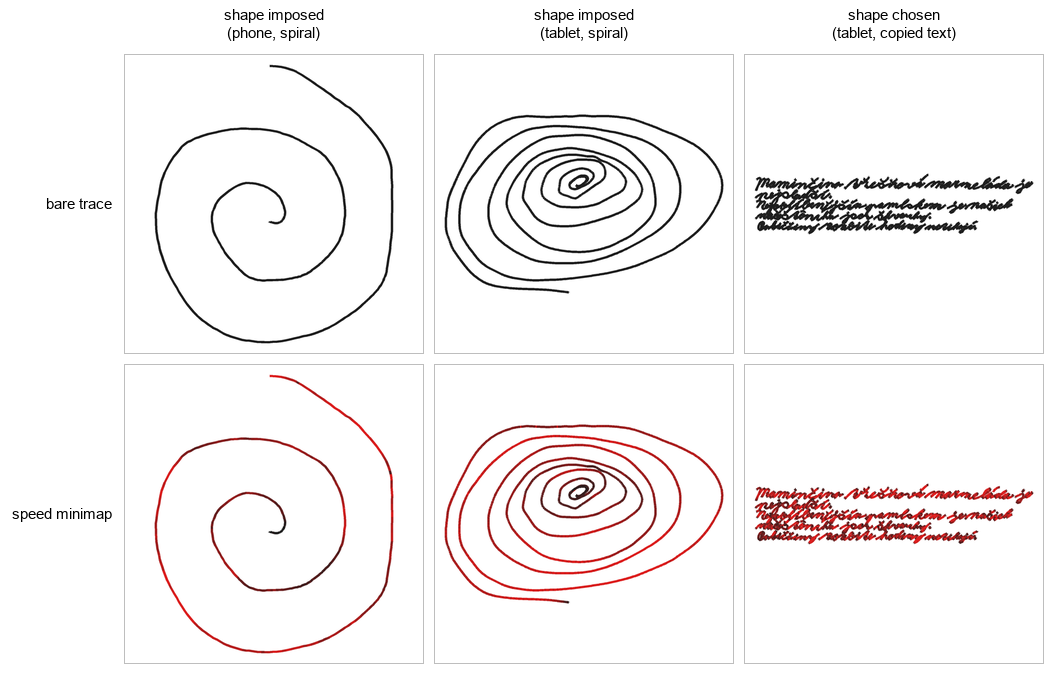
\includegraphics[width=\columnwidth]{figures/examples.png}
\end{center}
\caption{The same encoding on the two task regimes of \cref{sec:tasks}, read from recordings the
experiments actually used. Left and centre: the task prescribes the figure, so the bare trace is
nearly the same for everyone and what differs is the execution the colour carries. Right: a copied
text, where the produced shape already carries most of what distinguishes one recording from
another, and where the square canvas shrinks a wide multi-line page into a strip. No participant is
identified and no panel was chosen for its appearance.}
\label{fig:examples}
\end{figure}

Two properties matter for the argument. The normalisation uses no statistic of the cohort and no
label, so nothing about the class distribution can enter the image; and the mapping is
\emph{positional}, the only part of the pipeline that records where along the trace a value
occurred, which is what the controls of \cref{sec:results-controls} test directly.

\paragraph{Descriptor and model.} Unless stated otherwise, images are described by Local Phase
Quantisation (LPQ) \citep{ojansivu2008lpq} on each channel ($64 \times 64$, $5\times 5$ window,
$256$ bins per channel, $768$ dimensions, square-root transformed) and classified by a support
vector machine. A frozen ImageNet ResNet18 \citep{he2016resnet} with an $\ell_2$-regularised
logistic head is the second descriptor over the identical images, which separates the encoding's
contribution from the descriptor's.



%%%%%%%%%%%%%%%%%%%%%%%%%%%%%%%%%%%%%%%%%%%%%%%%%%%%%%%%%%%%%%%%%%%%%%%%%%%%%%%%%%%%%%%%%%%%%%%%
%% The experiments, as declared. Written 28 November 2026.
%% Every row of the table below is a directory in runs/ and a numbered script in scripts/; the
%% labels are the ones the protocol documents use, so a reader can go from a sentence here to the
%% addendum that fixed it and the run that produced it.
%%%%%%%%%%%%%%%%%%%%%%%%%%%%%%%%%%%%%%%%%%%%%%%%%%%%%%%%%%%%%%%%%%%%%%%%%%%%%%%%%%%%%%%%%%%%%%%%

\subsection{The experiments}
\label{sec:experiments}

Nine experiments, run in the order below, each fixed in a protocol document before it ran. Four are
the per-corpus chain the prior study defined; five were added as the study's own results forced
questions it could not answer, and each of those five carries a dated addendum that declares its
hypotheses with their direction before the run. The two layers that aggregate --- M1 and M2 ---
fit nothing: they re-analyse prediction files the earlier experiments archived.

\paragraph{E1, the encoding sweep.} Every encoding the corpus admits, under both geometries, on the
screening splits. Its purpose is to establish that the renderers read the corpus correctly and to
produce the per-task and per-participant predictions the later steps reuse. No claim is made from
it.

\paragraph{E2, selection inside training.} The encoding is chosen inside each outer training set by
inner-fold score, never on test scores and never on the corpus as a whole. What reaches the later
steps is therefore one arm per outer fold, which is what a practitioner would have.

\paragraph{E3, the competitive comparison.} Four pipelines on the same splits: the bare trace with
LPQ, the selected minimap with LPQ, a kinematic and pressure feature vector, and a frozen ImageNet
ResNet18. This is the comparison the prior paper reported on one corpus.

\paragraph{E4, confirmation.} The whole of E2 and E3 repeated on a disjoint master seed
(20261219) that no screening step ever touched. Every number this paper reports as a result comes
from this stage; E1--E3 exist to choose arms, not to support claims.

\paragraph{D1, the acquisition floor.} The two-feature probe of \cref{sec:floor}, run under the
identical protocol in every corpus with a participant endpoint, including the corpora where our own
arms are positive.

\paragraph{C1 and C2, the mechanism controls.} The circular shift along each stroke and the joint
permutation within each stroke, rendered and described identically to the real arm, under both
descriptors. They ask whether a gain depends on \emph{where} the painted value sits.

\paragraph{N1, the null-channel probe.} Three channels that carry nothing about the writer ---
acquisition order as a ramp, an AR(1) series whose lag-one autocorrelation is matched to the
recording's own, and white noise --- painted by the identical renderer. The controls above keep the
real values and move them; this one keeps the geometry and replaces the values, so it asks whether
a gain is the channel's \emph{content} or merely the presence of a varying channel. We are not
aware of this control being reported for this family of encodings.

\paragraph{F1, a baseline for each descriptor.} The same confirmation splits with each descriptor
scored against \emph{its own} bare trace, which separates a change of encoding from a change of
descriptor. This experiment was added after C2 showed that the headline margin of the prior study
spanned two descriptors at once.

\paragraph{G1, the split noise, measured.} Twenty fresh master seeds per corpus, to replace the
inherited $\pm 0.03$ band with a measurement, and to price what picking an arm on the split it is
scored on is worth.

\paragraph{M1, the corpus-level layer.} The six within-descriptor margins treated as one dataset of
six estimates with their own variances: pooled effect, heterogeneity, the binary corpus property as
a moderator, the six contrasts as one multiplicity family, and the minimum detectable effect of each
corpus.

\paragraph{M2, the task-level layer.} The same quantities with the task slot as the unit: thirty
slots, the equivalence outcome of each against the fixed margin, the task property estimated
\emph{within} corpora, and the variance of the margin between slots of one corpus against its
variance between corpora. This is the experiment the present framing turns on, and
\cref{sec:statistics} gives its registered plan in full.

\paragraph{What was deliberately not run.} No per-slot selection of the encoding, because selecting
inside a slot would widen the family and change the estimand; no per-slot acquisition floor, which
is possible and is left to future work (\cref{sec:future}); no re-tuning of any hyperparameter grid
per corpus; and no segmentation of the one corpus whose recordings carry no task boundaries, since
a segmentation tuned after seeing a score would compromise every other number here.


\subsection{Evaluation protocol}
\label{sec:protocol}


Every cohort is evaluated identically, and every decision --- inclusion rule, task definition,
contact rule, unit conversion, split design --- was written into a per-cohort protocol document
\emph{before} any classifier was fitted on that cohort. Where the direction of the study changed
mid-stream, the protocol carries a dated addendum, not a rewrite.

\paragraph{Partitions.} Five repeats of five stratified outer folds, three inner folds for
selection, nested so that representation and hyperparameters are chosen on training participants
only. \textbf{The participant is the unit}: all recordings of a participant are in the same fold,
and participant decisions are the majority vote over the available tasks. Screening and
confirmation use disjoint master seeds; we treat split-to-split variation of $\pm 0.03$ macro F1 as
noise, and report no gain that does not reappear on the confirmation seed. That band was inherited
rather than measured; \cref{sec:results-splitnoise} measures it on twenty fresh seeds per corpus
and reports where it is too narrow.

\paragraph{Statistics, within a cohort.} Confidence intervals are $10{,}000$ label-stratified
participant bootstrap resamples. Paired contrasts use participant-wise swap randomisation.
Multiplicity is corrected by the Holm procedure \citep{holm1979} within families declared in the
protocol.

\paragraph{Spatial controls.} To test whether a gain comes from \emph{where} the signal sits, we
apply two destructive controls at render time, each preserving every per-stroke marginal exactly:
a \emph{circular shift} of the signal values along each stroke, and a \emph{joint permutation} of
the signal values within each stroke. Both leave the ink and the colour histogram identical; only
the correspondence between position and value is destroyed.

\subsection{The acquisition floor}
\label{sec:floor}


\begin{definition}[Acquisition floor]
For a cohort $\mathcal{D}$ and an evaluation protocol $\Pi$, the acquisition floor
$\phi(\mathcal{D}, \Pi)$ is the score that $\Pi$ assigns to a classifier whose only inputs are
properties of the recording process that no behaviour of the subject can produce.
\end{definition}

We instantiate it with two features per recording: the \textbf{median sampling interval between
consecutive contact samples}, and $\log_{10}$ of the \textbf{first timestamp}, that is, the origin
of the session clock. Neither is a symptom: no disease makes a digitiser sample at $9$~ms instead
of $7$~ms, and none sets the clock. The second is independent of the writer by construction, the
first only approximately so, since a digitiser can drop samples under fast motion. That is one
reason to keep the probe to features whose dependence on behaviour is this weak, and to report wider
probes separately.

Either input can be a constant in a given release, and saying which is part of reading the floor:
the median interval varies in one of the six corpora here and the clock origin in three. Where
both are constant the floor is at chance by construction, and the cohort is clean of these two
artefacts by inspection of two columns: a stronger statement than a classifier at chance, not a
weaker one. Where one varies the floor is effectively a one-feature probe: the $0.929$ reported
below on \textsc{Drot\'ar--Dobe\v{s}} is the session clock alone.

The floor is not chance: chance is a property of the label distribution, while the floor is a
property of the dataset as assembled and is the level below which a score is uninformative about the
phenomenon. We therefore report the margin $\Delta_\phi = \text{score} - \phi$ for every arm and
cohort, and treat it rather than the score as the quantity that carries evidence.

Measuring it costs nothing: it reuses the protocol already in place, and the features are two
reductions over a timestamp column. We report it for all six cohorts with a participant endpoint,
including those where our own results are positive.

\subsection{Use of generative AI}
\label{sec:genai}

Generative AI assistance was used in preparing this work and is disclosed here as the journal
requires. A large language model (Anthropic Claude) was used as a coding and editing assistant:
writing and reviewing analysis and rendering code, drafting and copy-editing the manuscript,
checking every bibliographic record against a registry, and auditing the reported numbers against
the run artefacts that produced them. It was not used to design the study, to choose hypotheses or
task subsets, to generate or impute data, or to interpret results; the protocol documents that fix
every design decision predate it and are dated. All code was executed by the authors, all outputs
were reviewed by the authors, and the authors take full responsibility for the content.
% Confirmed by the corresponding author on 2026-11-24 as matching how the tool was actually used
% across the project. Re-check before submission only if another tool is brought in, or if the
% division of labour changes during revision.




%%%%%%%%%%%%%%%%%%%%%%%%%%%%%%%%%%%%%%%%%%%%%%%%%%%%%%%%%%%%%%%%%%%%%%%%%%%%%%%%%%%%%%%%%%%%%%%%
%% Results --- what was measured, without inference. Written 28 November 2026.
%%
%% Deliberately descriptive: point estimates, counts and intervals, no verdict and no reading.
%% Every inferential statement about these numbers is in sec-statistics.tex, which also carries
%% the plan that was registered before any of them existed.
%%
%% Sources, cell by cell:
%%   headline / within / controls / signature / splitnoise / diagramo ... tables/ (generated)
%%   corpus-level margins and floors ..... runs/across_cohorts/per_cohort.csv
%%   null channel ........................ runs/zhu/n1_null_confirmation
%%   task level .......................... runs/task_level/{per_slot,pooled}.csv
%%   variance components ................. runs/across_cohorts/variance_components.csv
%%%%%%%%%%%%%%%%%%%%%%%%%%%%%%%%%%%%%%%%%%%%%%%%%%%%%%%%%%%%%%%%%%%%%%%%%%%%%%%%%%%%%%%%%%%%%%%%

\section{Results}
\label{sec:results}

This section reports what was measured. It states point estimates, counts and intervals and draws
no conclusion from them: every test, every verdict against a registered threshold and every
statement of the form ``therefore'' belongs to \cref{sec:statistics}, which also carries the
analysis plan as it was registered before these numbers existed. The separation is deliberate, and
it is how the reader can see which quantities were produced by the runs and which by the analysis.

\subsection{The competitive comparison, corpus by corpus}
\label{sec:results-headline}

\Cref{tab:headline} gives the four pipelines on the confirmation splits with the participant as the
unit, together with each corpus's acquisition floor. Read as a margin of the best minimap arm over
the bare trace, the corpora fall into a wide range: $+0.334$ on the full ParkinsonHW release,
$+0.252$ on Zhu, $+0.168$ on the clean ParkinsonHW sub-cohort, $+0.050$ on DiaGraMo, $+0.015$ on
Character Trajectories, $+0.010$ on Drot\'ar--Dobe\v{s} and $+0.002$ on PaHaW.

Four of those seven best arms are the frozen-backbone arm rather than the texture-descriptor arm, so
four of those margins change the descriptor at the same time as the encoding.
\Cref{tab:within} therefore gives each descriptor its own bare-trace baseline on the same splits.
Under LPQ the margins are $+0.086$ (ParkinsonHW, clean), $+0.109$ (Zhu), $+0.010$
(Drot\'ar--Dobe\v{s}), $+0.008$ (Character Trajectories), $+0.002$ (PaHaW) and $-0.021$ (DiaGraMo).
Under the frozen backbone they are $+0.014$, $-0.014$, $-0.063$, $+0.001$, $+0.011$ and $-0.011$.
The largest positive margin under the backbone in any corpus of this study is $+0.014$.

The descriptor swap on the identical bare trace is worth $+0.154$ on the clean ParkinsonHW
sub-cohort and $+0.265$ on Zhu, and $-0.015$ on PaHaW.

\begin{table}[t]
\caption{Macro F1 at the unit level on the confirmation splits, which no model or encoding choice ever saw. $\Delta$ is the gain of the best minimap arm over the static trace; \emph{kinem.} is the 83 kinematic and pressure attributes computed from the same signals; \emph{floor} is the two-number acquisition classifier of \cref{sec:floor}, which contains no handwriting at all. $\Delta_\phi$, the margin over that floor, is the quantity that carries evidence: the score alone does not.}
\label{tab:headline}
\vskip 0.1in
\begin{center}
\begin{small}
\begin{tabular}{lrrrrrr}
\toprule
cohort & static & minimap & $\Delta$ & kinem. & floor & $\Delta_\phi$ \\
\midrule
ParkinsonHW$^{\dagger}$ & 0.757 & 0.925 & $+0.168$ & 0.854 & 0.666 & $+0.259$ \\
Zhu et al. & 0.627 & 0.879 & $+0.252$ & 0.843 & 0.473 & $+0.406$ \\
DiaGraMo & 0.658 & 0.708 & $+0.050$ & 0.716 & 0.453 & $+0.256$ \\
Drot\'ar--Dobe\v{s} & 0.767 & 0.777 & $+0.010$ & 0.783 & 0.929 & $-0.152$ \\
PaHaW & 0.634 & 0.636 & $+0.002$ & 0.650 & 0.642 & $-0.006$ \\
Char.\ Trajectories & 0.982 & 0.996 & $+0.015$ & 0.998 & 0.501 & $+0.495$ \\
\bottomrule
\end{tabular}
\end{small}
\end{center}
\vskip -0.1in
\end{table}

%% Generated by scripts/x3_paper_tables.py from runs/. Do not edit by hand.
%% Every number below comes from the run that produced it. An edit here is silently overwritten
%% the next time the generator runs, and breaks the guarantee that no number in the paper can
%% differ from its run. To change a number, change the run or the generator.
\begin{table*}[t]
\caption{Each descriptor against its own bare trace, on the confirmation splits: the first three columns LPQ, the next three the frozen ResNet18, each $\Delta$ a minimap arm minus the static trace \emph{under the same descriptor and model grid}. \emph{descr.}\ is the remaining ingredient of the headline margin --- the identical bare trace, read by the backbone instead of by LPQ. Only the backbone's static arm is new; the other three reproduce \cref{tab:headline} exactly, on the same splits. Hypotheses, thresholds and the cohorts that can decompose into anything were registered before the run (addendum~F).}
\label{tab:within}
\vskip 0.1in
\begin{center}
\begin{small}
\begin{tabular}{lrrrrrrr}
\toprule
 & \multicolumn{3}{c}{LPQ} & \multicolumn{3}{c}{frozen ResNet18} & \\
\cmidrule(lr){2-4} \cmidrule(lr){5-7}
cohort & static & minimap & $\Delta$ & static & minimap & $\Delta$ & descr. \\
\midrule
ParkinsonHW$^{\dagger}$ & 0.757 & 0.843 & $+0.086$ & 0.911 & 0.925 & $+0.014$ & $+0.154$ \\
Zhu et al. & 0.627 & 0.736 & $+0.109$ & 0.893 & 0.879 & $-0.014$ & $+0.265$ \\
DiaGraMo & 0.658 & 0.637 & $-0.021$ & 0.720 & 0.708 & $-0.011$ & $+0.061$ \\
Drot\'ar--Dobe\v{s} & 0.767 & 0.777 & $+0.010$ & 0.825 & 0.762 & $-0.063$ & $+0.058$ \\
PaHaW & 0.634 & 0.636 & $+0.002$ & 0.619 & 0.630 & $+0.011$ & $-0.015$ \\
Char.\ Trajectories & 0.982 & 0.989 & $+0.008$ & 0.995 & 0.996 & $+0.001$ & $+0.013$ \\
\bottomrule
\end{tabular}
\end{small}
\end{center}
\vskip -0.1in
\end{table*}


\subsection{The acquisition floor}
\label{sec:results-floor}

The two-feature probe reaches $0.97$ within the \texttt{hw\_dataset} block of the ParkinsonHW
release and $0.93$ on Drot\'ar--Dobe\v{s}, where it is above every real arm in \cref{tab:headline}.
On PaHaW it reaches $0.642$. On the clean ParkinsonHW sub-cohort it is $0.666$; on Zhu $0.473$, on
DiaGraMo $0.453$ and on Character Trajectories $0.501$. In the last three both probe features are
constant in the release, so the probe is at chance by construction. On Drot\'ar--Dobe\v{s} the
median sampling interval is constant and the score is the session clock alone.

\subsection{The mechanism controls}
\label{sec:results-controls}

\Cref{tab:controls} gives the two destructive controls. Where the minimap arm carries a margin,
shifting the painted signal along each stroke costs between $0.06$ and $0.11$ macro F1; where it
carries none, the same operation moves the score by at most $0.03$. The within-stroke joint
permutation behaves in the same direction on the same corpora.

The null-channel probe was run on Zhu, on the confirmation splits. Under LPQ the bare trace reaches
$0.6272$ and the real speed channel $0.7362$; acquisition order reaches $0.6561$, the
smoothness-matched AR(1) $0.6125$ and white noise $0.6154$. Under the frozen backbone the same five
arms reach $0.8926$, $0.8787$, $0.9137$, $0.8860$ and $0.8996$.

\begin{table}[t]
\caption{Spatial controls on the LPQ selection arm, screening splits. Both destroy only the correspondence between position along the stroke and signal value, leaving the ink, the contact mask and every per-stroke marginal identical. A cost means the classifier reads \emph{where} the signal sits along the trace; no cost means it reads only how the values are distributed.}
\label{tab:controls}
\vskip 0.1in
\begin{center}
\begin{small}
\begin{tabular}{lrrrrr}
\toprule
cohort & minimap & shift & permuted & $\delta$ shift & $\delta$ perm. \\
\midrule
ParkinsonHW$^{\dagger}$ & 0.738 & 0.637 & 0.624 & $-0.101$ & $-0.114$ \\
Zhu et al. & 0.750 & 0.688 & 0.649 & $-0.062$ & $-0.101$ \\
DiaGraMo & 0.645 & 0.669 & 0.648 & $+0.024$ & $+0.003$ \\
Drot\'ar--Dobe\v{s} & 0.783 & 0.758 & 0.772 & $-0.025$ & $-0.011$ \\
PaHaW & 0.590 & 0.586 & 0.607 & $-0.004$ & $+0.017$ \\
Char.\ Trajectories & 0.989 & 0.985 & 0.989 & $-0.004$ & $+0.000$ \\
\bottomrule
\end{tabular}
\end{small}
\end{center}
\vskip -0.1in
\end{table}


\subsection{The within-corpus task contrast on DiaGraMo}
\label{sec:results-diagramo}

DiaGraMo is the only corpus that elicits both kinds of task from the same children on the same
display in the same session. Over its ten figure-imposed slots the minimap margin is $+0.030$, and
over its four shape-informative slots $+0.069$ (\cref{tab:diagramo}). Against a bare trace
described by the frozen backbone rather than by LPQ, no task set of this corpus shows a positive
margin.

\begin{table*}[t]
\caption{The contrast inside DiaGraMo: the same children, the same tablet, the same session. Ten tasks impose the target figure, four do not, and the direction was registered before the splits were drawn. It came out backwards, and the \emph{nuisance} column --- six acquisition descriptors, no handwriting in them --- shows why that outcome cannot be read as evidence about pen dynamics.}
\label{tab:diagramo}
\vskip 0.1in
\begin{center}
\begin{small}
\begin{tabular}{lrrrrrr}
\toprule
task set & static & LPQ & ResNet18 & $\Delta$ best & floor & nuisance \\
\midrule
all 14 tasks & 0.658 & 0.637 & 0.708 & $+0.050$ & 0.453 & 0.784 \\
graphomotor (10) & 0.616 & 0.599 & 0.647 & $+0.030$ & 0.432 & 0.593 \\
writing (4) & 0.635 & 0.623 & 0.703 & $+0.069$ & 0.424 & 0.846 \\
\bottomrule
\end{tabular}
\end{small}
\end{center}
\vskip -0.1in
\end{table*}


\subsection{Split-to-split variation, measured}
\label{sec:results-splitnoise}

Twenty fresh master seeds per corpus give half-widths of the margin from $0.0021$ to $0.0556$,
tracking the size of the smaller class rather than the corpus (\cref{tab:splitnoise}). Picking the
arm on the split it is scored on is worth up to $+0.028$ on one corpus and nothing on five.

\begin{table*}[t]
\caption{Split noise, measured rather than assumed (Addendum G). The confirmation design re-run on twenty fresh master seeds per cohort, features reused so that only the fold assignment varies, and the minimap arm held at the one that cohort's confirmation reported so that no seed can re-select it. \emph{Half-width} is half the 5th--95th interval, which is the quantity the $\pm 0.03$ band of \cref{sec:protocol} asserts without measuring: it is too narrow on \textsc{Zhu} and \textsc{ParkinsonHW} and conservative elsewhere, and it tracks the size of the smaller class rather than the cohort. $^{\dagger}$As in \cref{tab:headline}, \textsc{ParkinsonHW} is read on its clean sub-cohort; the full release, which \cref{sec:floor} excludes, measures 0.052. Two reported margins fall outside their own interval: \textsc{Character Trajectories} above it by $0.001$, which 853 units make almost unavoidable, and \textsc{Drot\'ar--Dobe\v{s}} below it by $0.006$, the one case with substance. The reported numbers are not replaced by any column here; the rule for reading them was fixed before the seeds ran.}
\label{tab:splitnoise}
\vskip 0.1in
\begin{center}
\begin{small}
\begin{tabular}{llrrrcr}
\toprule
cohort & descriptor & reported $\Delta$ & seed mean & sd & 5th--95th & half-width \\
\midrule
ParkinsonHW$^{\dagger}$ & ResNet18 & $+0.168$ & $+0.145$ & 0.035 & [$+0.093$, $+0.204$] & 0.056 \\
Zhu et al. & ResNet18 & $+0.252$ & $+0.230$ & 0.022 & [$+0.192$, $+0.254$] & 0.031 \\
DiaGraMo & ResNet18 & $+0.050$ & $+0.037$ & 0.015 & [$+0.018$, $+0.057$] & 0.020 \\
Drot\'ar--Dobe\v{s} & LPQ & $+0.010$ & $+0.032$ & 0.012 & [$+0.016$, $+0.049$] & 0.017 \\
PaHaW & LPQ & $+0.002$ & $-0.006$ & 0.023 & [$-0.037$, $+0.022$] & 0.030 \\
Char.\ Trajectories & ResNet18 & $+0.015$ & $+0.012$ & 0.001 & [$+0.010$, $+0.014$] & 0.002 \\
\bottomrule
\end{tabular}
\end{small}
\end{center}
\vskip -0.1in
\end{table*}


\subsection{The corpus as the unit}
\label{sec:results-corpus-layer}

Treated as six estimates with their own variances (\cref{tab:across,tab:pooled}), the within-descriptor
margins pool to $+0.017$ under LPQ with a $95\,\%$ interval of $[-0.029, +0.063]$,
$\hat\tau = 0.031$, $I^2 = 65\,\%$ and a prediction interval of $[-0.078, +0.113]$. Under the frozen
backbone they pool to $-0.008$ with $\hat\tau = 0.014$ and $I^2 = 48\,\%$; restricted to the four
corpora above their floor, the backbone pools to $+0.001$ with $\hat\tau = 0$ and $I^2 = 0\,\%$.

The binary corpus property --- whether the task fixes the figure --- carries a coefficient of
$+0.098$ and leaves $0.009$ of the $0.031$ heterogeneity. Its observed assignment is the most
extreme of the $15$ available, exact $p = 0.067$, which is the smallest value $1/15$ permits.

Each corpus could have detected, at $80\,\%$ power, a margin of $0.127$ (ParkinsonHW, clean),
$0.109$ (Zhu), $0.066$ (PaHaW), $0.052$ (Drot\'ar--Dobe\v{s}), $0.038$ (DiaGraMo) and $0.006$
(Character Trajectories). The pooled estimate of $+0.017$ is below five of those six values.

Decomposed over corpus, master seed and repeat, the standard deviation of the margin is $0.0372$
between corpora, $0.0179$ between master seeds within a corpus and $0.0369$ between repeats within
a seed.

%% Generated by scripts/x3_paper_tables.py from runs/. Do not edit by hand.
%% Every number below comes from the run that produced it. An edit here is silently overwritten
%% the next time the generator runs, and breaks the guarantee that no number in the paper can
%% differ from its run. To change a number, change the run or the generator.
\begin{table*}[t]
\caption{The six within-descriptor margins under LPQ as one family (Addendum~H). $\Delta_w$ and its interval are the cohort's own, from $10{,}000$ participant bootstrap resamples; $p$ is participant-wise swap randomisation; \emph{$p$ Holm, six} corrects across the six cohorts rather than inside each one, which is the family this study actually ran. MDE$_{80}$ is the margin that cohort could have detected at $80\,\%$ power given its own standard error --- the quantity that separates \emph{no effect was found} from \emph{none could have been}. Note the two rows that disagree with each other: \textsc{Character Trajectories} is the most significant contrast in the family at a margin of $+0.008$, and \textsc{ParkinsonHW} is eleven times larger and fails it, separated by nothing but $853$ units against $51$.}
\label{tab:across}
\vskip 0.1in
\begin{center}
\begin{small}
\begin{tabular}{llrrcrrr}
\toprule
cohort & figure fixed & units & $\Delta_w$ & 95\,\% CI & $p$ & $p$ Holm, six & MDE$_{80}$ \\
\midrule
ParkinsonHW$^{\dagger}$ & yes & 51 & $+0.086$ & [$-0.002$, $+0.176$] & 0.0647 & 0.2588 & 0.127 \\
Zhu et al. & yes & 58 & $+0.109$ & [$+0.036$, $+0.189$] & 0.0061 & 0.0305 & 0.109 \\
DiaGraMo & no & 273 & $-0.021$ & [$-0.048$, $+0.005$] & 0.1241 & 0.3723 & 0.038 \\
Drot\'ar--Dobe\v{s} & no & 120 & $+0.010$ & [$-0.026$, $+0.047$] & 0.5807 & 1.0000 & 0.052 \\
PaHaW & no & 75 & $+0.002$ & [$-0.045$, $+0.048$] & 0.9854 & 1.0000 & 0.066 \\
Char.\ Trajectories & no & 853 & $+0.008$ & [$+0.004$, $+0.012$] & 0.0001 & 0.0006 & 0.006 \\
\bottomrule
\end{tabular}
\end{small}
\end{center}
\vskip -0.1in
\end{table*}

%% Generated by scripts/x3_paper_tables.py from runs/. Do not edit by hand.
%% Every number below comes from the run that produced it. An edit here is silently overwritten
%% the next time the generator runs, and breaks the guarantee that no number in the paper can
%% differ from its run. To change a number, change the run or the generator.
\begin{table*}[t]
\caption{Pooling the six margins, and why the pooled number is the wrong summary (Addendum~H). Random effects by REML with a Hartung--Knapp interval, fixed in the protocol before the run because the method-of-moments estimator is biased downward at six studies. $\hat\tau$ is the between-cohort standard deviation and the last column is the prediction interval for a new cohort. The declared threshold was $\hat\tau \ge 0.03$ with $I^2 \ge 50\,\%$: the LPQ rows meet it and the backbone rows do not, so under a frozen ImageNet descriptor the six cohorts are \emph{one} effect and above the floor that effect is $+0.001$. \emph{DL} is DerSimonian--Laird beside the declared estimator, printed because on the first and third rows the $\hat\tau$ arm of that threshold is met by REML and not by DL, so those two verdicts rest on an estimator choice made in advance; $I^2$ and $Q$ do not depend on it, and they are what the conclusion rests on. The moderator of \cref{sec:when} --- whether the task fixes the figure --- is worth $+0.098$ and leaves $0.009$ of the $0.031$ heterogeneity; its assignment of two cohorts to the figure-fixed group is the most extreme of the $15$ available, exact $p = 0.067$, which is the smallest value $1/15$ permits and is therefore reported as an extremity rather than as significance.}
\label{tab:pooled}
\vskip 0.1in
\begin{center}
\begin{small}
\begin{tabular}{lrrcrrrc}
\toprule
set & $k$ & pooled & 95\,\% CI & $\hat\tau$ & DL & $I^2$\,\% & prediction interval \\
\midrule
LPQ, all six & 6 & $+0.017$ & [$-0.029$, $+0.063$] & 0.0307 & 0.0208 & 65 & [$-0.078$, $+0.113$] \\
LPQ, all six, seed weights & 6 & $+0.030$ & [$-0.024$, $+0.085$] & 0.0482 & 0.0348 & 89 & [$-0.116$, $+0.176$] \\
LPQ, above the floor & 4 & $+0.035$ & [$-0.062$, $+0.132$] & 0.0537 & 0.0298 & 79 & [$-0.231$, $+0.300$] \\
LPQ, above the floor, seed weights & 4 & $+0.043$ & [$-0.056$, $+0.142$] & 0.0599 & 0.0499 & 94 & [$-0.247$, $+0.334$] \\
ResNet18, all six & 6 & $-0.008$ & [$-0.033$, $+0.016$] & 0.0139 & 0.0137 & 48 & [$-0.054$, $+0.038$] \\
ResNet18, above the floor & 4 & $+0.001$ & [$-0.001$, $+0.003$] & 0.0000 & 0.0000 & 0 & [$-0.003$, $+0.005$] \\
\bottomrule
\end{tabular}
\end{small}
\end{center}
\vskip -0.1in
\end{table*}


\subsection{The task as the unit}
\label{sec:results-task-layer}

\Cref{tab:tasklevel} gives all thirty slots. Two carry a margin whose $90\,\%$ interval clears
$+0.03$: the static spiral of the clean ParkinsonHW sub-cohort, $+0.152$ with interval
$[+0.070, +0.236]$, and the spiral of Zhu, $+0.119$ with $[+0.042, +0.200]$. The companion slot of
each of those two corpora is smaller: the dynamic spiral of ParkinsonHW is $+0.007$ and the Zhu wave
is $+0.060$, the latter with an interval of $[+0.004, +0.118]$.

Six slots have a $90\,\%$ interval contained in $\pm 0.03$: three graphomotor and writing slots of
DiaGraMo --- small spiral fast $+0.001$, lower loops fast $+0.006$, copy $+0.001$ --- and the three
character pairs, $+0.004$, $+0.001$ and $+0.020$. The remaining twenty-two slots have intervals that
cross one of the two margins. Three slots have an interval entirely below zero without reaching
$-0.03$: the big spiral, the saw and the rainbow slots of DiaGraMo, at $-0.033$, $-0.028$ and
$-0.043$.

Eight of PaHaW's slots lie between $-0.025$ and $+0.048$. Its spiral, the only slot of that corpus
whose figure is imposed, is $+0.016$.

Pooled over the thirty slots (\cref{tab:taskpooled}) the margin is $+0.000$ with a $95\,\%$ interval
of $[-0.008, +0.009]$, $\hat\tau = 0.0118$ and $I^2 = 53\,\%$. Split by the task property, the
fifteen figure-imposed slots pool to $-0.001$ with $\hat\tau = 0.0212$ and $I^2 = 65\,\%$, and the
fifteen shape-informative slots to $+0.005$ with $\hat\tau = 0.0055$ and $I^2 = 17\,\%$. Under the
frozen backbone the thirty slots pool to $+0.000$ with $\hat\tau = 0$ and $I^2 = 0\,\%$. Dropping
PaHaW leaves $-0.000$ over twenty-two slots; dropping the corpus whose floor exceeds its best real
arm leaves $+0.000$ over twenty-nine.

Estimated with corpus fixed effects, the task property carries a coefficient of $-0.0090$. Of the
$8{,}008$ assignments the restricted enumeration admits, $3{,}128$ are at least as extreme as the
observed one, exact $p = 0.391$, against an attainable minimum of $0.00012$. The unrestricted
permutation over all thirty slots gives $-0.0103$ with $p = 0.158$ of $100{,}000$ draws.

The heterogeneity of the thirty slots decomposes into $\hat\tau = 0.0098$ between slots within a
corpus and $\hat\tau = 0.0067$ between corpora. The median sampling standard deviation of a single
slot is $0.0164$.

Minimum detectable effects at $80\,\%$ power range from $0.003$ (the \textit{o}/\textit{a} pair of
Character Trajectories) to $0.142$ (the static spiral of ParkinsonHW). Twenty-six of the thirty
slots have an MDE$_{80}$ above $0.03$.

%% Generated by scripts/x3_paper_tables.py from runs/. Do not edit by hand.
%% Every number below comes from the run that produced it. An edit here is silently overwritten
%% the next time the generator runs, and breaks the guarantee that no number in the paper can
%% differ from its run. To change a number, change the run or the generator.
\begin{table}[t]
\caption{The thirty task slots, each estimated on its own (Addendum~I). \emph{Shape} is the property fixed in the protocol before any slot was computed: \emph{imp.} when every participant produces the same prescribed figure, \emph{inf.} when the produced shape varies with the content. $n$ is participants contributing to that slot, one recording each, so the participant fusion of the earlier protocol does not enter. \emph{static} and \emph{minimap} are participant-level macro F1 under LPQ on the confirmation splits, the minimap arm being the encoding selected inside the cohort's outer training folds --- never inside the slot. The interval is the \emph{90\,\%} one the two one-sided tests read, and the outcome is declared against the fixed margin $\delta = 0.03$: \emph{superior} when the lower bound clears $+\delta$, \emph{equivalent} when the whole interval lies inside $\pm\delta$, \emph{inconclusive} otherwise --- which is a statement about precision, not about equality. The last column is the margin that slot could have detected at 80\,\% power. Of the 15 imposed slots 2 are superior; of the 15 informative slots 4 are equivalent. $^{\dagger}$the clean sub-cohort, as everywhere in this paper.}
\label{tab:tasklevel}
\vskip 0.1in
\begin{center}
\setlength{\tabcolsep}{2.5pt}
\begin{footnotesize}
\begin{tabular}{llllrrrcll}
\toprule
cohort & slot & shape & $n$ & static & minimap & $\Delta_w$ & 90\,\% CI & outcome & MDE$_{80}$ \\
\midrule
ParkinsonHW$^{\dagger}$ & static spiral & imp. & 51 & 0.655 & 0.807 & $+0.152$ & [$+0.070$, $+0.236$] & \textbf{superior} & 0.142 \\
 & dynamic spiral & imp. & 47 & 0.821 & 0.828 & $+0.007$ & [$-0.072$, $+0.075$] & inconclusive & 0.127 \\
Zhu et al. & spiral & imp. & 58 & 0.662 & 0.782 & $+0.119$ & [$+0.042$, $+0.200$] & \textbf{superior} & 0.136 \\
 & wave & imp. & 58 & 0.660 & 0.720 & $+0.060$ & [$+0.004$, $+0.118$] & inconclusive & 0.096 \\
DiaGraMo & RCFT recognition & inf. & 270 & 0.583 & 0.575 & $-0.008$ & [$-0.031$, $+0.015$] & inconclusive & 0.040 \\
 & RCFT recall & inf. & 271 & 0.583 & 0.575 & $-0.008$ & [$-0.036$, $+0.019$] & inconclusive & 0.047 \\
 & dictation & inf. & 260 & 0.600 & 0.615 & $+0.014$ & [$-0.004$, $+0.034$] & inconclusive & 0.033 \\
 & big spiral, fast & imp. & 272 & 0.503 & 0.470 & $-0.033$ & [$-0.060$, $-0.006$] & inconclusive & 0.046 \\
 & small spiral, fast & imp. & 273 & 0.517 & 0.517 & $+0.001$ & [$-0.023$, $+0.024$] & equivalent & 0.041 \\
 & saw, fast & imp. & 273 & 0.623 & 0.595 & $-0.028$ & [$-0.045$, $-0.011$] & inconclusive & 0.030 \\
 & upper loops, fast & imp. & 272 & 0.572 & 0.588 & $+0.015$ & [$-0.008$, $+0.038$] & inconclusive & 0.039 \\
 & lower loops, fast & imp. & 272 & 0.590 & 0.596 & $+0.006$ & [$-0.015$, $+0.027$] & equivalent & 0.035 \\
 & rainbow, fast & imp. & 271 & 0.604 & 0.561 & $-0.043$ & [$-0.066$, $-0.020$] & inconclusive & 0.039 \\
 & combined loops, fast & imp. & 273 & 0.515 & 0.527 & $+0.013$ & [$-0.014$, $+0.040$] & inconclusive & 0.046 \\
 & small spiral, precise & imp. & 273 & 0.604 & 0.593 & $-0.012$ & [$-0.033$, $+0.009$] & inconclusive & 0.036 \\
 & lower loops, precise & imp. & 273 & 0.604 & 0.586 & $-0.018$ & [$-0.039$, $+0.003$] & inconclusive & 0.036 \\
 & combined loops, precise & imp. & 273 & 0.529 & 0.521 & $-0.008$ & [$-0.035$, $+0.019$] & inconclusive & 0.046 \\
 & copy & inf. & 270 & 0.659 & 0.661 & $+0.001$ & [$-0.022$, $+0.025$] & equivalent & 0.040 \\
Drot\'ar--Dobe\v{s} & whole recording, unsegmented & inf. & 120 & 0.767 & 0.777 & $+0.010$ & [$-0.020$, $+0.041$] & inconclusive & 0.052 \\
PaHaW & spiral & imp. & 72 & 0.616 & 0.632 & $+0.016$ & [$-0.019$, $+0.050$] & inconclusive & 0.058 \\
 & letter l & inf. & 75 & 0.563 & 0.564 & $+0.002$ & [$-0.031$, $+0.033$] & inconclusive & 0.055 \\
 & bigram le & inf. & 75 & 0.570 & 0.573 & $+0.003$ & [$-0.029$, $+0.037$] & inconclusive & 0.056 \\
 & trigram les & inf. & 75 & 0.623 & 0.618 & $-0.006$ & [$-0.048$, $+0.038$] & inconclusive & 0.074 \\
 & word lektorka & inf. & 75 & 0.537 & 0.514 & $-0.023$ & [$-0.076$, $+0.029$] & inconclusive & 0.090 \\
 & word porovnat & inf. & 75 & 0.582 & 0.629 & $+0.048$ & [$-0.015$, $+0.111$] & inconclusive & 0.107 \\
 & word nepopadnout & inf. & 75 & 0.548 & 0.523 & $-0.025$ & [$-0.081$, $+0.029$] & inconclusive & 0.094 \\
 & sentence & inf. & 75 & 0.558 & 0.580 & $+0.021$ & [$-0.038$, $+0.080$] & inconclusive & 0.100 \\
Char.\ Traj. & u vs. v & inf. & 286 & 0.996 & 1.000 & $+0.004$ & [$+0.001$, $+0.009$] & equivalent & 0.007 \\
 & o vs. a & inf. & 312 & 0.993 & 0.994 & $+0.001$ & [$-0.001$, $+0.003$] & equivalent & 0.003 \\
 & m vs. n & inf. & 255 & 0.952 & 0.972 & $+0.020$ & [$+0.011$, $+0.030$] & equivalent & 0.016 \\
\bottomrule
\end{tabular}
\end{footnotesize}
\end{center}
\vskip -0.1in
\end{table}

%% Generated by scripts/x3_paper_tables.py from runs/. Do not edit by hand.
%% Every number below comes from the run that produced it. An edit here is silently overwritten
%% the next time the generator runs, and breaks the guarantee that no number in the paper can
%% differ from its run. To change a number, change the run or the generator.
\begin{table*}[t]
\caption{Pooling the thirty slots, with the registered test of the task property beside it (Addendum~I). Random effects by REML with a Hartung--Knapp interval, the same estimator the six-cohort layer used. The last column is the prediction interval for a new slot. Rows two and three are the sensitivity analyses the protocol declared, and the last row is the secondary estimand. \textbf{H14} required a within-cohort coefficient of at least $+0.050$ and a restricted permutation $p \le 0.05$; the coefficient is $-0.0090$ and the exact $p$ is $0.391$ of $8008$ enumerated assignments, whose attainable minimum is $0.00012$, so \textbf{H15 holds}: once the cohort is held fixed the task property does not account for the slot-level margins. The unrestricted permutation, which mixes the between-cohort differences back in, gives $-0.0103$ and $p = 0.158$ and is printed only for contrast. \textbf{H16} required at least $8$ of the $15$ informative slots to be declared equivalent; $4$ are, so \textbf{H17 holds}. The variance components measured but not tested: slot-to-slot variation inside a cohort is $\hat\tau = 0.0098$ against $\hat\tau = 0.0067$ between cohorts.}
\label{tab:taskpooled}
\vskip 0.1in
\begin{center}
\begin{small}
\begin{tabular}{lrrcrrc}
\toprule
set & $k$ & pooled & 95\,\% CI & $\hat\tau$ & $I^2$\,\% & prediction interval \\
\midrule
LPQ, all thirty slots & 30 & $+0.000$ & [$-0.008$, $+0.009$] & 0.0118 & 53 & [$-0.025$, $+0.026$] \\
LPQ, without PaHaW (tasks not blind) & 22 & $-0.000$ & [$-0.011$, $+0.011$] & 0.0135 & 64 & [$-0.030$, $+0.029$] \\
LPQ, without the cohort below its floor & 29 & $+0.000$ & [$-0.009$, $+0.009$] & 0.0122 & 55 & [$-0.026$, $+0.026$] \\
LPQ, figure imposed & 15 & $-0.001$ & [$-0.021$, $+0.019$] & 0.0212 & 65 & [$-0.050$, $+0.047$] \\
LPQ, shape informative & 15 & $+0.005$ & [$-0.000$, $+0.010$] & 0.0055 & 17 & [$-0.009$, $+0.019$] \\
ResNet18, all thirty slots & 30 & $+0.000$ & [$-0.000$, $+0.000$] & 0.0000 & 0 & [$-0.000$, $+0.000$] \\
\bottomrule
\end{tabular}
\end{small}
\end{center}
\vskip -0.1in
\end{table*}


\subsection{Reading and rendering verification}
\label{sec:results-svc}

All nine encodings render on SVC2004, whose seven-field specification is published and unambiguous
(\cref{tab:signature}). That corpus has no participant endpoint and no acquisition floor and
contributes to no estimate in this paper.

%% Generated by scripts/x3_paper_tables.py from runs/. Do not edit by hand.
%% Every number below comes from the run that produced it. An edit here is silently overwritten
%% the next time the generator runs, and breaks the guarantee that no number in the paper can
%% differ from its run. To change a number, change the run or the generator.
\begin{table}[t]
\caption{SVC2004 skilled-forgery verification, writer-independent, single held-out split. Reported apart from \cref{tab:headline} because this cohort has no participant endpoint and no acquisition floor: a forger and a genuine signer are not two groups of people. It is the cleanest case of a label the shape cannot carry, since the forgery copies the shape on purpose, and the static trace sits at chance while every encoding that carries a signal scores above it. A single split carries no interval, so the smallest of those margins should not be read as established.}
\label{tab:signature}
\vskip 0.1in
\begin{center}
\begin{small}
\begin{tabular}{lrrr}
\toprule
encoding & macro F1 & accuracy & ROC AUC \\
\midrule
static & 0.491 & 0.492 & 0.505 \\
S & 0.528 & 0.531 & 0.543 \\
P & 0.564 & 0.567 & 0.586 \\
A & 0.533 & 0.534 & 0.555 \\
Z & 0.533 & 0.534 & 0.557 \\
SPA & 0.581 & 0.583 & 0.617 \\
SPZ & 0.589 & 0.593 & 0.631 \\
SAZ & 0.576 & 0.580 & 0.618 \\
PAZ & 0.613 & 0.617 & 0.653 \\
\bottomrule
\end{tabular}
\end{small}
\end{center}
\vskip -0.1in
\end{table}



%%%%%%%%%%%%%%%%%%%%%%%%%%%%%%%%%%%%%%%%%%%%%%%%%%%%%%%%%%%%%%%%%%%%%%%%%%%%%%%%%%%%%%%%%%%%%%%%
%% The statistical analysis: the plan as registered, then applied. Written 28 November 2026.
%%
%% Every threshold quoted here is in protocols/PROTOCOL-common.md and was committed before the
%% quantity it judges existed. The commits are named in the text on purpose: for this journal the
%% audit trail is part of the method, not an appendix to it.
%%
%% Sources: runs/task_level/{per_slot,pooled,variance_components,moderator,equivalence}.*
%%          runs/across_cohorts/* for the corpus-level layer
%%%%%%%%%%%%%%%%%%%%%%%%%%%%%%%%%%%%%%%%%%%%%%%%%%%%%%%%%%%%%%%%%%%%%%%%%%%%%%%%%%%%%%%%%%%%%%%%

\section{Statistical analysis}
\label{sec:statistics}

The numbers of \cref{sec:results} are judged here, against thresholds that were written down before
those numbers existed. We give the plan first in each subsection and then apply it, because for
this study the order matters: the plan is version-controlled and dated, and the only reason its
verdicts can be taken at face value is that it could not have been written after the fact.

\subsection{How the plan was registered}
\label{sec:registration}

Each corpus has a protocol document fixing its inclusion rule, task definition, contact rule, unit
conversion and split design, committed before any classifier was fitted on that corpus. Where the
study's own results forced a question the protocol had not anticipated, the answer is a dated
addendum committed \emph{before} the run it governs, never a rewrite: addendum~B declared the
within-corpus task contrast of \cref{sec:results-diagramo}; C the control arms under the backbone;
E the null-channel probe; F the per-descriptor baseline; G the split-noise measurement; H the
corpus-level layer; and I the task-level layer of this section, committed as \texttt{4c3eb0e} at a
point when no per-slot quantity on the confirmation splits had been computed and the script that
computes them did not exist.

Three disclosures are part of the registration rather than of the discussion, because they bound
what the verdicts below can mean, and all three were written into addendum~I before it ran. First,
the direction of the task property is \emph{not} a blind prediction: it is this study's own
corpus-level ordering, restated as a model so that it could fail. Second, the two task sets of
DiaGraMo had already been compared under addendum~B and that comparison had already failed, so
addendum~I recorded in advance that H15 --- the null --- was the outcome it expected. Third, PaHaW's
tasks are not blind, since the prior single-corpus paper reported its endpoint over a subset of
slots; PaHaW is therefore carried in the primary analysis and removed again in a declared
sensitivity analysis.

\subsection{Within a corpus}
\label{sec:stats-within}

Intervals are $10{,}000$ label-stratified participant bootstrap resamples; paired contrasts use
participant-wise swap randomisation; all repeats of a participant move together, so no resample
splits a participant across arms. These are the same estimators, with the same seeds, as the prior
single-corpus study, and the task-level layer reuses them unchanged --- which is what makes its
regression control meaningful: the participant-level margin re-derived from the task-level
prediction files reproduces the archived value in all twelve corpus-by-descriptor cells to within
$5 \times 10^{-5}$.

\subsection{Equivalence, instead of a null result}
\label{sec:stats-equivalence}

\paragraph{The plan.} A margin that lands inside an interval containing zero is not evidence of
equivalence; it is also what too few participants look like. We therefore declared a margin
$\delta = 0.03$ macro F1 and two one-sided tests at $\alpha = 0.05$, which read the $90\,\%$
interval of a slot's margin \citep{schuirmann1987,lakens2018equivalence}. Each slot receives exactly
one of four outcomes: \emph{superior} when the lower bound clears $+\delta$, \emph{inferior} when
the upper bound falls below $-\delta$, \emph{equivalent} when the whole interval lies inside
$\pm\delta$, and \emph{inconclusive} otherwise. ``Inconclusive'' is a statement about precision and
is never reported as equality.

The margin is not a convenience. It is the band this project has used since the single-corpus work
to mean ``within split noise'', and \cref{sec:results-splitnoise} measures the half-widths that
justify it. One value is used for all thirty slots, because a margin taken from each slot's own
noise would make the threshold depend on the data it judges.

\paragraph{Applied.} Of the thirty slots, two are superior, six are equivalent, twenty-two are
inconclusive and none is inferior. \textbf{H16} required at least $8$ of the $15$
shape-informative slots to be declared equivalent; $4$ are, so \textbf{H17 holds}. The claim that
the encoding is demonstrably as good as the bare trace where the shape carries the label is
\emph{not} supported at this margin --- not because the margins there are large, but because eleven
of those fifteen slots cannot resolve $0.03$: twenty-six of the thirty slots have an
MDE$_{80}$ above the margin itself. The four slots that do support it are the three character
pairs, whose standard errors are an order of magnitude smaller than any clinical slot's, and the
copy slot of DiaGraMo.

This is the first place in this study where an equivalence claim was available to be made, and the
answer is that the data do not carry it. Every ``inside the $\pm 0.03$ band'' sentence in the
earlier framing of this work was a power statement.

\subsection{Pooling thirty slots nested in six corpora}
\label{sec:stats-pooling}

\paragraph{The plan.} Slot margins are pooled by random effects fitted with restricted maximum
likelihood and reported with a Hartung--Knapp interval \citep{hartung2001}, fixed in advance because
the method-of-moments estimator is biased downward at this number of studies
\citep{viechtbauer2005}. We report $\hat\tau$, $I^2$ \citep{higgins2002} and a prediction interval
beside every pooled point, because a pooled point summarises an effect only if there is one effect.
Thirty slots measured on six groups of people are not thirty independent units, so heterogeneity is
decomposed: the same estimator with an intercept gives the total, and with corpus fixed effects ---
which absorb every between-corpus difference --- gives what remains between slots of one corpus.

\paragraph{Applied.} Over the thirty slots the pooled margin is $+0.000$, interval
$[-0.008, +0.009]$, with $\hat\tau = 0.0118$ and $I^2 = 53\,\%$. Neither sensitivity analysis moves
it: $-0.000$ without PaHaW, $+0.000$ without the corpus whose floor exceeds its best real arm.
Under the frozen backbone the thirty slots are one effect of $+0.000$ with $\hat\tau = 0$.

The decomposition is the result of this subsection, and it was measured rather than tested, as
addendum~I declared. Between slots of one corpus $\hat\tau = 0.0098$; between corpora
$\hat\tau = 0.0067$. \textbf{Task-to-task variation inside a corpus is larger than
corpus-to-corpus variation}, and both are smaller than the median sampling standard deviation of a
single slot, $0.0164$. The heterogeneity that the corpus-level layer attributed to differences
between corpora ($\hat\tau = 0.031$, $I^2 = 65\,\%$) does not survive being asked at which level it
lives.

One consequence of the change of unit must be stated and was not registered, so we flag it as an
unregistered observation: pooling slots weights a corpus by how many tasks it administered, so
DiaGraMo contributes fourteen units and Drot\'ar--Dobe\v{s} one. The slot-level pooled estimate of
$+0.000$ and the corpus-level $+0.017$ are therefore not competing estimates of one quantity; they
are two different estimands, and which one answers a question depends on whether the question is
about corpora or about tasks.

\subsection{The task property, tested within corpora}
\label{sec:stats-moderator}
%% Alias for the labels the shared generated tables reference. tables/*.tex are emitted by
%% scripts/x3_paper_tables.py for all three builds and their captions cite the earlier
%% draft's section names; aliasing here keeps one generator for three documents instead of
%% branching it per document.
\label{sec:when}

\paragraph{The plan.} The corpus-level test of this property is bounded by arithmetic: with six
corpora and two on one side, the exact permutation cannot return a $p$ below $1/15 = 0.067$, which
addendum~H stated in advance and never called significance. The task-level test is not bounded that
way. The property is entered in a meta-regression \emph{with corpus fixed effects}, so the
coefficient is a within-corpus contrast and no between-corpus difference can reach it, and it is
tested by a \textbf{restricted permutation} that holds each corpus's number of figure-imposed slots
fixed and re-labels only inside corpora. Only PaHaW, one of eight, and DiaGraMo, ten of fourteen,
vary under it, giving $\binom{8}{1}\binom{14}{10} = 8{,}008$ assignments, enumerated exactly, with
an attainable minimum $p$ of $0.00012$. The weights are held at the fitted model's, which is the
standard permutation of a meta-regression coefficient and is recorded as an implementation choice.
\textbf{H14} required both a coefficient $\ge +0.05$ and $p \le 0.05$.

\paragraph{Applied.} The coefficient is $-0.0090$ and $3{,}128$ of the $8{,}008$ assignments are at
least as extreme as the observed one, exact $p = 0.391$. \textbf{H15 holds}, in both of its
conditions and with the sign reversed from the prediction. Once the corpus is held fixed, whether
the task imposes the figure does not account for the slot-level margins. The unrestricted
permutation, which mixes the between-corpus differences back in, gives $-0.0103$ and $p = 0.158$;
it is reported for contrast and was declared as such.

The two sides of the property differ, but not in the way the hypothesis named: the fifteen
figure-imposed slots are \emph{heterogeneous} around zero ($-0.001$, $\hat\tau = 0.0212$,
$I^2 = 65\,\%$) while the fifteen shape-informative slots are \emph{homogeneous} and slightly
positive ($+0.005$, $\hat\tau = 0.0055$, $I^2 = 17\,\%$). Where the figure is imposed the encoding
sometimes does a great deal and usually nothing; where the shape carries the label it reliably does
almost nothing. That is a different statement from the one we registered, it is not a test, and
\cref{sec:discussion} treats it as the hypothesis for another study rather than as a result of this
one.

\subsection{Multiplicity}
\label{sec:stats-multiplicity}

\paragraph{The plan.} Holm correction \citep{holm1979} within families declared in the protocol.
The thirty slot contrasts are one such family, declared in addendum~I, and are corrected as one ---
the family this study actually ran, rather than one family per corpus.

\paragraph{Applied.} Five of the thirty randomisation $p$ values are below $0.05$ uncorrected.
\textbf{After Holm over the thirty, exactly one survives, and it is the smallest margin of the
five}: the \textit{m}/\textit{n} character pair, $+0.020$, adjusted $p = 0.003$ --- a contrast whose
magnitude is inside the equivalence margin. The two slots the equivalence procedure calls superior
do not survive: the static spiral of ParkinsonHW, $+0.152$, has an adjusted $p$ of $0.123$, and the
Zhu spiral, $+0.119$, of $0.549$.

The pairing is worth naming, because it is the whole argument of this section in two rows of a
table. The largest effects in the study are the least certain, and the only certain one is too small
to matter. The superiority verdicts in \cref{tab:tasklevel} are uncorrected by construction --- the
equivalence procedure reads an interval, not a corrected $p$ --- and a reader who wants a
multiplicity-controlled claim about those two spirals does not have one here.

\subsection{Power, reported with every null}
\label{sec:stats-power}

\paragraph{The plan.} For every unit we report MDE$_{80}$, the margin it could have detected at
$80\,\%$ power and two-sided $5\,\%$ given its own standard error. A null above a unit's
MDE$_{80}$ is an absence of evidence; a null below it is evidence of absence. Without the column a
reader cannot tell which one they are looking at, and this study has published both kinds.

\paragraph{Applied.} At corpus level, five of the six corpora could not have detected the pooled
margin of $+0.017$; only Character Trajectories, with $853$ recordings of one writer, could. At slot
level, twenty-six of the thirty slots could not have detected the equivalence margin of $0.03$. The
eight PaHaW slots need between $0.055$ and $0.108$; the two ParkinsonHW slots $0.142$ and $0.127$;
the two Zhu slots $0.136$ and $0.096$. The clinical corpora in this literature, at the sizes they
are released in, are not instruments that can resolve effects of the size this recipe produces.

\subsection{Screening and confirmation as a two-stage design}
\label{sec:stats-twostage}

\paragraph{The plan.} The two master seeds form a two-stage design whose interim rule was fixed
before either stage ran: a representation reaches confirmation only if it leads at screening, and no
margin is reported as a gain unless it reappears on the confirmation seed inside the declared band.
We claim \emph{no} propagation of $\alpha$ between the stages --- they are separate families and the
confirmation intervals are not widened for having passed a screen.

\paragraph{Applied.} What the screen can buy is measured instead of argued: picking the arm on the
split it is scored on is worth up to $+0.028$ on one corpus and nothing on five. Every number in
\cref{sec:results} is from the confirmation stage, and the task-level layer draws no new split at
all --- it re-slices the confirmation predictions, so it inherits that stage's separation rather
than creating a third one.

\subsection{What the registrations predicted, and what happened}
\label{sec:stats-ledger}

Nine hypotheses were registered with a direction and a threshold, across addenda~B, C, E, F, H and
I. \textbf{Three held.} H6, the null-channel probe: the gain on Zhu is the channel's content and not
the mere presence of a varying channel. H10, heterogeneity between corpora under LPQ. H12, the
corpus-level moderator --- at a $p$ equal to its attainable minimum, which is why it is reported as
an extremity and not as significance.

\textbf{Six failed.} H1 and H2, the within-corpus task contrast on DiaGraMo, with the sign reversed.
H4, the spatial controls under the frozen backbone, where the test dissolved its own target because
the backbone had no margin left for a control to destroy. H8, that at least half of a reported
margin survives a descriptor-matched baseline --- refused on all three corpora that had a margin to
decompose. H14, the task property within corpora. H16, equivalence on the shape-informative slots.

We report the ledger rather than only its favourable rows because the ledger is the result. A study
of this shape earns its conclusions from the registrations that failed, and this one has more of
those than of the other kind.


%%%%%%%%%%%%%%%%%%%%%%%%%%%%%%%%%%%%%%%%%%%%%%%%%%%%%%%%%%%%%%%%%%%%%%%%%%%%%%%%%%%%%%%%%%%%%%%%
%% Discussion, limitations and future work. Written 28 November 2026.
%%
%% The sample-size figures of sec:future come from runs/task_level/per_slot.csv:
%% n_required = n_units * (mde80 / 0.03)^2, the usual inverse-square scaling of a standard error.
%% Median over the twenty-seven clinical slots is 480, range 256 to 1,187.
%%%%%%%%%%%%%%%%%%%%%%%%%%%%%%%%%%%%%%%%%%%%%%%%%%%%%%%%%%%%%%%%%%%%%%%%%%%%%%%%%%%%%%%%%%%%%%%%

\section{Discussion}
\label{sec:discussion}

\subsection{Does the encoding transfer?}
\label{sec:discussion-transfer}

Narrowly, and to two tasks. The published single-corpus result does reappear outside the corpus it
came from: on the clean ParkinsonHW sub-cohort and on Zhu the minimap arm beats the bare trace
under the same descriptor by $+0.086$ and $+0.109$, and the mechanism controls put that gain where
the encoding puts it --- destroying \emph{where} the painted value sits removes it, while painting a
channel with no information about the writer does not reproduce it. Both of those corpora prescribe
the figure, and in both the gain is carried by a single slot: the static spiral and the drawn
spiral, $+0.152$ and $+0.119$, while their companion slots give $+0.007$ and $+0.060$. A reader who
wants the one-sentence answer should have this one: the effect is real, it is localised to one task
in each of two corpora, and over the thirty tasks of this study it pools to zero.

Three qualifications belong in the same breath, because each of them was measured rather than
suspected. The margins reported for this recipe are in good part a change of descriptor: the
identical bare trace read by ImageNet features instead of by LPQ is worth $+0.154$ and $+0.265$ on
those two corpora, and under the backbone no corpus here gains more than $+0.014$ from the encoding.
Neither of the two superior slots survives Holm correction over the thirty-slot family, while the
one contrast that does survive is $+0.020$ --- inside the margin we declared as noise. And the
corpus that carries the largest raw margin of all, the full ParkinsonHW release at $+0.334$, is the
one whose capture metadata alone reaches $0.97$.

\subsection{The rule we registered does not hold at the task level}
\label{sec:discussion-rule}

The ordering that motivated this study --- the encoding helps where the task fixes the figure and
not where the produced shape carries the label --- holds across corpora and fails inside them. With
corpus fixed effects the task property is worth $-0.0090$ with $p = 0.391$ over an exact enumeration
whose attainable minimum is $0.00012$. This is the second time this study has asked that question
with the instrument that can answer it and received a no; the first was the within-corpus contrast on
DiaGraMo, declared with its direction and failed with the sign reversed.

We take the consequence rather than the escape. The between-corpus ordering is real in the sense
that it describes the six corpora, but what it tracks is not the task property alone: across corpora
the instrument, the recruitment, the population and the task all move together, and the component
that survives being isolated is not the task. The honest reading of the corpus-level moderator ---
coefficient $+0.098$, nine tenths of the heterogeneity absorbed, $p$ at its attainable minimum --- is
that it is a good description of six points, not a tested mechanism.

What replaces it is weaker and, we think, more useful. The two sides of the property differ in
\emph{dispersion} rather than in mean: the figure-imposed slots are heterogeneous around zero
($\hat\tau = 0.021$, $I^2 = 65\,\%$), the shape-informative slots homogeneous and nearly flat
($\hat\tau = 0.006$, $I^2 = 17\,\%$). Imposing the figure appears to be a necessary condition for a
large margin and nowhere near a sufficient one: ten of DiaGraMo's imposed slots produce nothing, and
three of them are reliably negative. That is a hypothesis for a study designed around it, and it is
stated here as one.

\subsection{Task-to-task variation exceeds corpus-to-corpus variation}
\label{sec:discussion-unit}

The quantitative result we did not expect is the variance decomposition. Between slots of one corpus
$\hat\tau = 0.0098$; between corpora $\hat\tau = 0.0067$. Both are below the median sampling
standard deviation of a single slot. A field that asks ``does representation $X$ work on dataset
$Y$'' is asking about the smaller of the two components, with an instrument whose noise exceeds
both.

This has a direct methodological consequence, and it is the one we would most like to be carried
forward: the task, not the corpus, is the natural unit for claims of this kind. It is also almost
free to adopt. The thirty estimates here were produced without rendering an image, fitting a model
or drawing a split; they are a re-slice of prediction files that any pipeline of this shape already
writes. The per-task breakdown is what shows that two corpus-level successes are two task-level
successes, which is not the same claim and not the one a reader of the corpus-level table would
infer.

\subsection{Equivalence was not available to be claimed}
\label{sec:discussion-equivalence}

We set out to test whether the encoded image is \emph{as good as} the bare trace where the shape
already carries the label, and the answer is that these corpora cannot say. Four of fifteen
shape-informative slots are equivalent at $\delta = 0.03$; eleven are inconclusive, and twenty-six
of the thirty slots overall have a minimum detectable effect larger than the margin itself. Three of
the four that do resolve belong to a non-clinical corpus with one writer.

We report this as a failure of H16 and not as a null finding, because the distinction is the point.
``No difference was found'' and ``the difference was shown to be smaller than $0.03$'' are different
claims, and only the second is a result. The earlier framing of this work made the first kind of
statement repeatedly, in the form of margins declared to be inside a $\pm 0.03$ band; every one of
those was a statement about our precision rather than about the representation.

\subsection{What a reader should take to the next cohort}
\label{sec:discussion-practice}

Five things, none of them expensive, and all of them things this study got wrong before it got them
right. Report the corpus's acquisition floor, so a score has a reference point; two of the corpora
here are partly or wholly separable from capture metadata, and one of them is the corpus the
original result came from. Give each descriptor its own bare-trace baseline, so a margin is about
the channel and not about the features. Report what effect the unit could have detected, so that a
null can be read at all. Measure the split noise instead of inheriting a band. And break the
endpoint down by task, because a corpus-level margin can be one task's margin diluted by seven
others --- or, as on DiaGraMo, a mixture of positive and reliably negative slots that averages to
nothing.

\subsection{Limitations}
\label{sec:limitations}

Thirty slots are not thirty independent units: fourteen come from one corpus and eight from
another, so the within-corpus component of the variance decomposition is estimated mainly inside
DiaGraMo, and the restricted permutation draws its variation from only two corpora. The
Drot\'ar--Dobe\v{s} recordings carry no task boundaries, so the second dysgraphia cohort contributes
one slot and cannot inform the within-corpus contrast at all. The acquisition floor is carried as a
corpus attribute rather than re-estimated per slot, which is a measurement this layer does not have.
Character Trajectories has a single writer, so its three slots support no participant-level claim
and enter as recording-level units. PaHaW's task subset was chosen in earlier work, so its eight
slots are not blind; the primary and the PaHaW-free analyses agree, which is why the verdicts stand.
The moderator's direction was informed by our own corpus-level results, as the registration states.
Pooling slots weights a corpus by how many tasks it administered, which makes the slot-level and
corpus-level pooled estimates two estimands rather than two estimates. And the selected
representation is chosen inside each corpus's training folds, not inside a slot, so a slot's margin
is the corpus's chosen arm evaluated there --- deliberately, since selecting per slot would widen
the family, but it means a slot-specific encoding might do better than any number here.

Finally, the screening of \cref{sec:screening} is a limitation as much as a method. Nineteen of
twenty-seven candidate corpora could not be obtained by download, and the eight that could are not a
random sample of handwriting research; they are the corpora whose authors chose open deposition.

\subsection{Future work}
\label{sec:future}

\paragraph{Corpora sized for the question.} The most actionable number in this paper is a design
number. Scaling each slot's standard error by the usual inverse square root, resolving a margin of
$0.03$ at $80\,\%$ power would take a median of $480$ participants per task across the twenty-seven
clinical slots here, with a range from $256$ to $1{,}187$; seventeen of those twenty-seven would
need more than twice the participants they have. The largest clinical corpus in this study has
$273$. Until collections of that size exist, work in this area can report effects and should not
report equivalence, and a study that wants to compare two representations on one clinical task needs
to say in advance what effect it could see.

\paragraph{A corpus built for the contrast.} The scarce resource in this design is a corpus that
elicits both kinds of task from the same participants on the same device in the same session. There
are two here, and one of them contributes a single figure-imposed slot. A prospective collection
that administers a balanced battery --- the same participants, half imposed figures and half free
content --- would test the task property with the confound held fixed by construction rather than by
a fixed effect, and it is the one experiment that could overturn the verdict of
\cref{sec:stats-moderator}.

\paragraph{A floor per task.} The acquisition floor is currently a corpus attribute. Computing it
per slot would show whether the capture artefacts that make two of these corpora partly separable
are spread across their battery or concentrated in particular tasks, which would change how a
contaminated corpus is salvaged: a corpus with a clean subset of tasks is more useful than a corpus
discarded whole.

\paragraph{Task boundaries in the unsegmented corpus.} Locating the elicited tasks inside the
Drot\'ar--Dobe\v{s} recordings would turn one slot into five and would be the first independent test
of the task-level contrast outside DiaGraMo. It must be done as its own study, with the
segmentation fixed before any score is computed, because a segmentation tuned against a metric would
compromise every number that depends on it.

\paragraph{Selection inside the task.} The arms here are the corpus's chosen encoding evaluated per
slot. Whether choosing the encoding \emph{per task}, inside training folds, recovers more than the
corpus-level choice is a well-posed question with a declared family size, and it is the one
extension of the method itself that these results suggest is worth the multiplicity it costs.


\section{Conclusions}
\label{sec:conclusions}

A published single-corpus result was treated as a hypothesis and tested on corpora of the same data
format, with one frozen pipeline and every decision registered in advance. It transfers, narrowly:
under a descriptor-matched baseline the encoding is worth $+0.086$ and $+0.109$ on two Parkinson
corpora whose task prescribes the figure, the mechanism controls localise that gain to where the
painted value sits, and a channel carrying no information about the writer does not reproduce it.

Taking the task as the unit shows what that sentence conceals. The two corpus-level gains are two
task-level gains --- a static spiral at $+0.152$ and a drawn spiral at $+0.119$ --- and over the
thirty tasks of six corpora the encoding pools to $+0.000$. Neither of the two survives Holm
correction over the family this study ran; the one contrast that does is $+0.020$, inside the margin
we declared as noise. The task property we registered to explain where the encoding helps does not
explain it within a corpus: $-0.009$, exact $p = 0.391$ over an enumeration whose attainable minimum
is $0.00012$. And the variance of the margin between tasks of one corpus exceeds its variance
between corpora, which makes the corpus the wrong unit for the question the field asks of it.

We could not claim equivalence. Four of fifteen tasks whose shape carries the label are
demonstrably as good as the bare trace at a margin of $0.03$; eleven cannot resolve that margin, and
twenty-six of the thirty tasks have a minimum detectable effect larger than it. Resolving $0.03$ on
a clinical task at $80\,\%$ power would take a median of $480$ participants, against the $273$ of
the largest clinical corpus available to us. That is the finding we would most like to see acted on:
for effects of this size, the public corpora of this field are not yet instruments that can measure
them, and a study that reports ``no difference'' on one of them is reporting its own precision.

What we would ask of the next paper in this line is short, and every item is something this study
had to learn. Report the corpus's acquisition floor, so a score has a reference point. Give each
descriptor its own baseline, so a margin is about the channel and not the features. Report the effect
the unit could have detected. Break the endpoint down by task. Register the direction before drawing
the splits, and publish the registrations that failed --- of the nine registered here with a
direction and a threshold, three held and six did not, and the six are where this paper's
conclusions come from.


\section*{Back matter}

\paragraph{Supplementary Materials.} Not applicable. The appendices below carry the arm-by-arm
results, the geometry sweep, the mechanism controls and the split-noise measurement.

\paragraph{Author Contributions.}
% [AUTHOR VERIFICATION REQUIRED]: CRediT roles are the authors' to assign. The draft below is a
% starting point, not a record; confirm or replace every role before submission.
Conceptualization, M.G.J.\ and \'A.S.; methodology, M.G.J.; software, M.G.J.; validation, M.G.J.,
\'A.S.\ and Y.M.G.C.; formal analysis, M.G.J.; investigation, M.G.J.; data curation, M.G.J.;
writing---original draft preparation, M.G.J.; writing---review and editing, \'A.S., Y.M.G.C.,
I.S.W., A.F.R.C.\ and J.G.S.S.; visualization, M.G.J.; supervision, \'A.S.\ and Y.M.G.C.; project
administration, Y.M.G.C.; funding acquisition, Y.M.G.C.\ and \'A.S. All authors have read and
agreed to the published version of the manuscript.

\paragraph{Funding.} This research was financed in part by the Coordena\c{c}\~ao de
Aperfei\c{c}oamento de Pessoal de N\'ivel Superior --- Brasil (CAPES) --- Finance Code 001, and by
a CAPES PDSE scholarship (process 88881.266133/2026-01). \'A.~S\'anchez acknowledges the support
from Spanish State Research Agency project no.\ PID2025-169751OB-I00.
% Both numbers supplied by the authors on 2026-11-24 from the VISAPP 2027 camera-ready, and the
% wording is that paper's. One thing left to check against the funder rather than against us:
% Spanish AEI grants often require their own acknowledgement formula, which can include the funder
% identifier MICIU/AEI/10.13039/501100011033. MDPI also asks for the standard funder spelling from
% search.crossref.org/funding. If the AEI formula applies, this is the sentence to extend.

\paragraph{Institutional Review Board Statement.} Ethical review and approval were waived for this
study because it is a secondary analysis of previously published, de-identified datasets that their
authors released for research use; no data were collected from human participants for this work.
Ethical approval for each original data collection was obtained by the authors of the corresponding
dataset and is reported in their respective publications.
% [AUTHOR VERIFICATION REQUIRED]: confirm this wording with the institution, and confirm that every
% cohort's release permits secondary analysis of this kind.

\paragraph{Informed Consent Statement.} Not applicable. No participants were recruited for this
study; informed consent for the original recordings was obtained by the investigators who collected
each dataset.

% The DOI strings are long and unbreakable, so this paragraph is set sloppy rather than left to
% overflow the margin.
\begingroup\sloppy
\paragraph{Data Availability Statement.} No new recordings were created. All seven cohorts are
third-party datasets, cited in \cref{sec:cohorts} and reached through their own providers:

\begin{itemize}\setlength{\itemsep}{0pt}
\item \textsc{ParkinsonHW} --- \url{https://doi.org/10.24432/C5Q01S}
\item \textsc{Character Trajectories} --- \url{https://doi.org/10.24432/C58G7V}
\item \textsc{DiaGraMo} --- \url{https://doi.org/10.5281/zenodo.21236910}
\item \textsc{Drot\'ar--Dobe\v{s}} --- \url{https://doi.org/10.1038/s41598-020-78611-9}
\item \textsc{Zhu} --- \url{https://doi.org/10.1371/journal.pone.0327733}
\item \textsc{PaHaW} --- \url{https://doi.org/10.1016/j.artmed.2016.01.004}
\item \textsc{SVC2004} --- \url{https://cse.hkust.edu.hk/svc2004/}
\end{itemize}

\noindent The recordings are not ours to redistribute and are
obtained from their original providers under those providers' terms. The analysis code, the
per-cohort protocol documents that register every design decision and its date, and the aggregate
result tables are available at \url{https://github.com/munifgebara/handwriting-acquisition-floor-paper}.
Per-participant predictions are not published.
% [AUTHOR VERIFICATION REQUIRED]: two things before submission. (1) PaHaW and some other releases
% are obtained on request from their authors rather than downloaded; state each cohort's actual
% access route. (2) MDPI requires that links to preregistered analysis plans be given in the
% manuscript. The protocol documents are the preregistration here, and they must be reachable at
% the URL above by the time this is submitted.
\endgroup

\paragraph{Acknowledgments.} During the preparation of this manuscript the authors used Anthropic
Claude for code authoring and review, manuscript drafting and copy-editing, bibliographic
verification and auditing of reported numbers against the run artefacts, as described in
\cref{sec:genai}. The authors have reviewed and edited the output and take full responsibility for
the content of this publication.

\paragraph{Conflicts of Interest.} The authors declare no conflict of interest. The funders had no
role in the design of the study; in the collection, analyses or interpretation of data; in the
writing of the manuscript; or in the decision to publish the results.


% Flush every pending float before the references begin, so that nothing from the body can land
% among them.


\clearpage
\bibliography{main}
\bibliographystyle{unsrtnat}

\end{document}
